\documentclass[
    oldfontcommands,
    sumario=abnt-6027-2012,
    12pt,
    openright,
    oneside,
    a4paper,
    chapter=TITLE,
    section=TITLE,
    english,
    brazil
]{abntex2mod}

% Pacotes e configurações
% Pacotes básicos
\usepackage{lmodern}
\usepackage[T1]{fontenc}
\usepackage[utf8]{inputenc}
\usepackage{lastpage}
\usepackage{indentfirst}
\usepackage{color,xcolor}
\usepackage{graphicx}
\usepackage{microtype}

% Glossário
\usepackage[subentrycounter,seeautonumberlist,nonumberlist=true]{glossaries}

% Citações e referências (ABNT, sistema numérico)
\usepackage[num,
	    abnt-repeated-author-omit=no,
	    abnt-url-package=url,
	    abnt-etal-list=0,
	    abnt-etal-text=emph,
	    abnt-thesis-year=both,
	    ]{abntex2cite}
\usepackage{lipsum}
\citebrackets()

% Matemática, tabelas, figuras e referências cruzadas
\usepackage[portuguese,onelanguage]{algorithm2e}
\usepackage{amsbsy}
\usepackage{amscd}
\usepackage{amsmath}
\usepackage{amssymb}
\usepackage{amsthm}
\usepackage{hyperref}
\usepackage{cleveref}
\usepackage{dsfont}
\usepackage{listings}
\usepackage{mathabx}
\usepackage{pdfpages}
\usepackage[font=default]{caption}
\usepackage{float}
\usepackage{multirow}
\usepackage{anyfontsize}

% Hiperlinks
\usepackage{hyperref}
\usepackage{url}
\usepackage{xcolor}
\newcommand{\link}[1]{{\color{blue}\href{#1}{#1}}}

% O memoir já define framed, shaded etc., e o xwatermark tenta redefini-los
\let\framed\undefined
\let\endframed\undefined
\let\shaded\undefined
\let\endshaded\undefined
\let\leftbar\undefined
\let\endleftbar\undefined
\let\snugshade\undefined
\let\endsnugshade\undefined

% Marca d'água da capa
\usepackage[printwatermark]{xwatermark}
\usepackage{transparent}
\newwatermark[pages=1,xpos=60pt,ypos=-180pt]{\transparent{0.2}
\includegraphics[width=.9\textwidth]{src/unesplogo.jpg}}

% Teoremas
\theoremstyle{plain}
\newtheorem{theorem}{Teorema}
\newtheorem{lemma}{Lema}
\providecommand*{\lemmaautorefname}{Lema}
\newtheorem{proposition}{Proposição}
\providecommand*{\propositionautorefname}{Proposição}
\newtheorem{corollary}{Corolário}
\providecommand*{\corollaryautorefname}{Corolário}
\newtheorem{conjecture}{Conjectura}
\providecommand*{\conjectureautorefname}{Conjectura}
\newtheorem{definition}{Definição}
\providecommand*{\definitionautorefname}{Definição}
\newtheorem{notation}{Notação}
\providecommand*{\notationautorefname}{Notação}
\newtheorem{remark}{Observação}
\providecommand*{\remarkautorefname}{Observação}
\newtheorem{example}{Exemplo}
\providecommand*{\exampleautorefname}{Exemplo}
\newtheorem{note}{Nota}
\providecommand*{\noteautorefname}{Nota}

% Listings
\lstset{
  language=C++,
  basicstyle=\ttfamily,
  keywordstyle=\color{blue},
  stringstyle=\color{verde},
  commentstyle=\color{red},
  extendedchars=true,
  showspaces=false,
  showstringspaces=false,
  numbers=left,
  numberstyle=\tiny,
  breaklines=true,
  backgroundcolor=\color{green!10},
  breakautoindent=true,
  fontadjust=false
}

% Cores e informações do PDF
\definecolor{blue}{RGB}{41,5,195}
\definecolor{verde}{rgb}{0,0.5,0}
\makeatletter
\hypersetup{
  pdftitle={\@title},
  pdfauthor={\@author},
  pdfcreator={LaTeX with unesp-abnTeX2},
  pdfkeywords={abnt}{latex}{abntex}{abntex2}{trabalho acadêmico},
  colorlinks=true,
  linkcolor=blue,
  citecolor=blue,
  filecolor=magenta,
  urlcolor=blue,
  bookmarksdepth=4
}
\makeatother

% Comandos globais
\everymath{\displaystyle}
\renewcommand{\sin}{\mathrm{sen}}
\renewcommand{\tan}{\mathrm{tg}}
\renewcommand{\csc}{\mathrm{cossec}}
\renewcommand{\cot}{\mathrm{cotg}}
\DeclareMathOperator{\posto}{\mathrm{posto}}
\DeclareMathOperator{\conv}{\mathrm{conv}}
\DeclareMathOperator{\diag}{\mathrm{diag}}
\DeclareMathOperator{\argmin}{\mathrm{arg}\min}
\DeclareMathOperator{\argmax}{\mathrm{arg}\max}

% Parágrafos
\setlength{\parindent}{2.0cm}
\setlength{\parskip}{0.2cm}

% Subfiguras
\newsubfloat{figure}
\providecommand*{\subfigureautorefname}{Subfigura}

% Atalhos
\newcommand{\FX}{\mathcal{F}(X)}
\newcommand{\F}{\ensuremath{\mathcal{F}}}
\newcommand{\R}{\ensuremath{\mathds{R}}}
\newcommand{\Aa}{[A]^{\alpha}}

% Citação em sobrescrito
\newcommand{\citep}[1]{\textsuperscript{\cite{#1}}}


% Caminho das figuras de resultados
\graphicspath{{./}{figuras/}}

\begin{document}

\selectlanguage{brazil}
\frenchspacing
% =========================
% ELEMENTOS PRÉ-TEXTUAIS
% =========================

\pretextual

\begin{table}[!t]
    \centering
    \begin{tabular}{lcr}
      \multirow[c]{3}{2cm}{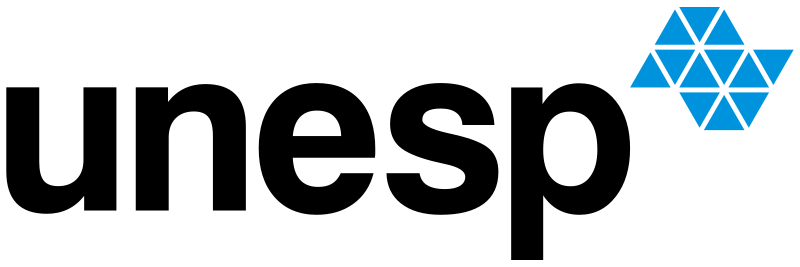
\includegraphics[width=.15\textwidth]{src/logounesp.png}}   & \textbf{\textsf{UNIVERSIDADE ESTADUAL PAULISTA}} & \multirow[c]{3}{1cm}{
\includegraphics[width=.1\textwidth]{src/igcelogo.jpg}} \\
      & \textbf{\textsf{ ``JÚLIO DE MESQUITA FILHO"}}  & \\
      & \textbf{\textsf{\footnotesize INSTITUTO DE GEOCIÊNCIAS E CIÊNCIAS EXATAS}}  & \\
    \end{tabular}

    \vspace{96pt}

\end{table}

\begin{center}
    \textbf{\Large RELATÓRIO}

\vspace{12pt}

    Bacharelado em Ciências da Computação\\
    Disciplina: Mineração de Dados e Aprendizado de Máquina
\end{center}

\vspace{60pt}

\begin{table}[!htb]
    \centering
    \begin{tabular}{|>{\centering\arraybackslash}p{.9\textwidth}|}
    \hline
    \vspace{24pt}
    METODOLOGIAS PARA EXTRAÇÃO DE CONHECIMENTO: \\
    PROCESSO KDD APLICADO ÀS BASES \\
    BREAST CANCER WISCONSIN E WINE \\
    \vspace{24pt}

    Eric Monteiro Perdigão\\
    Náthaly Emanuelle Silva Souza\\
    Victor Hugo da Maceno Terato\\
    Vitor Marchini Rolisola\\

    \vspace{36pt}
    Prof. Dr. Emilio Bergamim Júnior
    \vspace{36pt} \\
    \hline
    \end{tabular}

    \vspace{24pt}

\end{table}

\begin{center}
    Rio Claro (SP)

    \vspace{12pt}

    2026
\end{center}

\begin{resumo}[RESUMO]

Este relatório descreve a aplicação das sete etapas do processo de descoberta de conhecimento em bases de dados (\textit{Knowledge Discovery in Databases}, KDD) a dois conjuntos de dados com atributos contínuos e rótulos discretos: o \textit{Breast Cancer Wisconsin (Diagnostic)}, com 569 amostras, 30 atributos e duas classes (maligno e benigno), e o \textit{Wine}, com 178 amostras, 13 atributos e três classes (cultivares). Após a verificação da qualidade dos dados, a análise de \textit{outliers}, a padronização e a redução de dimensionalidade por Análise de Componentes Principais (PCA), foram aplicados algoritmos de agrupamento (K-Médias e DBSCAN), tratados como o caso-limite em que nenhum ponto é rotulado, e algoritmos de classificação semi-supervisionada (\textit{Self-Training} com Regressão Logística, \textit{Label Spreading} e \textit{Label Propagation}), variando a taxa de pontos rotulados de 5\% a 70\% e usando o KNN e a Regressão Logística como \textit{baselines}. No Wine, o \textit{Self-Training} atingiu F1-macro de 0,980 com apenas 5\% dos rótulos (7 amostras), superando a Regressão Logística de forma estatisticamente significativa (teste de Wilcoxon, $p = 0{,}008$). No Breast Cancer, cuja fronteira entre as classes é essencialmente linear, os métodos semi-supervisionados não apresentaram vantagem estatisticamente sustentada sobre a Regressão Logística treinada apenas com os pontos rotulados. Os resultados indicam que o benefício dos dados não rotulados depende da estrutura de agrupamento das classes, e que essa estrutura pode ser diagnosticada previamente pelo desempenho do K-Médias.

\vspace{\onelineskip}

\noindent
\textbf{Palavras-chave}: Mineração de dados. KDD. Aprendizado semi-supervisionado. Agrupamento. Breast Cancer Wisconsin. Wine.

\end{resumo}


\pdfbookmark[0]{\contentsname}{toc}
\renewcommand*\contentsname{SUMÁRIO}
\tableofcontents*
\cleardoublepage

% =========================
% ELEMENTOS TEXTUAIS
% =========================

\textual

\chapter[Introdução]{INTRODUÇÃO}

\section{CONTEXTO DO TRABALHO}

A mineração de dados (\textit{Data Mining}) corresponde, em geral, a uma etapa de um processo mais amplo de descoberta de conhecimento em bases de dados (\textit{Knowledge Discovery in Databases}, KDD), na qual os padrões presentes em um conjunto de dados são identificados e enumerados \citep{fayyad1996kdd}. O processo completo vai da compreensão do problema e da formulação de hipóteses até a interpretação dos resultados e o seu uso prático, e está próximo de outras metodologias consolidadas, como o CRISP-DM e o SEMMA \citep{azevedo2008kdd}.

Neste trabalho, as sete etapas do processo KDD propostas na disciplina de Mineração de Dados e Aprendizado de Máquina foram aplicadas a dois conjuntos de dados com \textbf{atributos contínuos e rótulos discretos}: o \textit{Breast Cancer Wisconsin (Diagnostic)} e o \textit{Wine}. Conforme a proposta do trabalho, foram descartados problemas que pudessem ser resolvidos com Regressão Linear ou Árvores de Decisão, e a investigação se concentrou em duas famílias de algoritmos:

\begin{itemize}
    \item \textbf{Classificação semi-supervisionada}, variando a taxa de pontos rotulados de 0,05 a 0,70, com o KNN (\textit{k-Nearest Neighbors}) e a Regressão Logística como \textit{baselines} de comparação;
    \item \textbf{Agrupamento}, com os algoritmos K-Médias e DBSCAN, vistos como o caso-limite em que nenhum ponto é rotulado.
\end{itemize}

\section{MOTIVAÇÃO}

Na maioria dos países, o câncer de mama é o tipo de câncer predominante entre as mulheres, e a probabilidade de cura é tanto maior quanto mais cedo a doença é detectada. Diversas abordagens estatísticas foram desenvolvidas para auxiliar essa detecção a partir de exames citopatológicos \citep{street1993nuclear, machinemantra_breast}. Nesse contexto, cada rótulo (benigno ou maligno) depende do laudo de um patologista, o que torna os dados rotulados caros. Esse é um cenário natural para o aprendizado com poucos rótulos.

Na vitivinicultura, garantir a autenticidade dos vinhos é um desafio: quanto mais precisa for a identificação da uva utilizada, maior é a garantia de qualidade e o controle contra fraudes. A classificação de vinhos a partir de sua composição química, seja pela cultivar, seja pela qualidade, é um problema clássico de ciência de dados \citep{girardi2025xwines, siddhardhan_wine}. Também aqui a rotulagem depende de análise especializada, e o aproveitamento de amostras não rotuladas pode reduzir o seu custo.

\section{OBJETIVOS}

O objetivo geral deste trabalho é medir quanto conhecimento sobre as classes pode ser extraído com supervisão parcial, desde \textbf{nenhum rótulo} (agrupamento) até \textbf{70\% de rótulos} (classificação semi-supervisionada), comparando os resultados com \textit{baselines} supervisionados que utilizam apenas os pontos rotulados.

Os objetivos específicos são:

\begin{itemize}
    \item Formular hipóteses verificáveis, com critérios objetivos, sobre a estrutura dos dois conjuntos de dados (Etapa 1);
    \item Selecionar, pré-processar e transformar os dados, justificando cada decisão (padronização, tratamento de \textit{outliers} e redução de dimensionalidade) com evidências empíricas (Etapas 2 a 4);
    \item Aplicar K-Médias e DBSCAN ao conjunto sem rótulos e avaliar a concordância dos agrupamentos com as classes reais (Etapa 5);
    \item Aplicar os métodos semi-supervisionados \textit{Self-Training}, \textit{Label Spreading} e \textit{Label Propagation} com taxas de rotulagem de 5\% a 70\%, comparando-os com o KNN e a Regressão Logística por meio de testes estatísticos pareados (Etapa 5);
    \item Interpretar os resultados, revisar as hipóteses iniciais e sintetizar o que os modelos revelam sobre os dados (Etapa 6), com recomendações práticas de uso (Etapa 7).
\end{itemize}

\section{ORGANIZAÇÃO DO RELATÓRIO}

O Capítulo 2 apresenta a fundamentação teórica do processo KDD e dos algoritmos utilizados. O Capítulo 3 descreve os materiais e métodos, que correspondem às Etapas 1 a 4 do KDD e ao protocolo experimental. O Capítulo 4 apresenta os resultados da mineração (Etapa 5). O Capítulo 5 reúne a avaliação e a interpretação dos resultados (Etapa 6) e o pós-processamento (Etapa 7). Por fim, o Capítulo 6 traz as considerações finais.

\chapter[Fundamentação Teórica]{FUNDAMENTAÇÃO TEÓRICA}

\section{O PROCESSO KDD}

O processo de descoberta de conhecimento adotado neste trabalho é dividido em sete etapas \citep{fayyad1996kdd, azevedo2008kdd}:

\begin{enumerate}
    \item \textbf{Compreensão do problema} e dos objetivos, com a formulação de hipóteses sobre o objeto de estudo;
    \item \textbf{Seleção} de um conjunto de dados relevante;
    \item \textbf{Pré-processamento}, que envolve limpeza, remoção de ruídos e normalização;
    \item \textbf{Transformação} dos dados para uma representação mais adequada, como na redução de dimensionalidade;
    \item \textbf{Mineração de dados}, isto é, a aplicação dos modelos de reconhecimento de padrões;
    \item \textbf{Avaliação e interpretação} dos resultados, que pode levar à revisão das hipóteses da Etapa 1;
    \item \textbf{Pós-processamento}, que depende dos objetivos e pode ser a redação de um artigo ou a implantação de um sistema.
\end{enumerate}

O processo não é necessariamente linear: a mineração pode contradizer as hipóteses iniciais e exigir que elas sejam repensadas. Além disso, os dados são compreendidos por meio dos modelos, de modo que a compreensão dos modelos é essencial para a compreensão dos dados.

\section{APRENDIZADO SEMI-SUPERVISIONADO}

No aprendizado semi-supervisionado, o conjunto de treino contém um pequeno subconjunto de pontos rotulados e um conjunto, em geral maior, de pontos não rotulados. A premissa central é a \textbf{hipótese de \textit{cluster}}: pontos próximos, ou ligados por regiões de alta densidade, tendem a compartilhar a mesma classe. Quando essa hipótese vale, os pontos não rotulados revelam a forma das classes e ajudam a posicionar a fronteira de decisão.

\subsection{SELF-TRAINING}

O \textit{Self-Training} \citep{yarowsky1995unsupervised} é um método envoltório (\textit{wrapper}): um classificador base é treinado com os pontos rotulados e, a cada iteração, os pontos não rotulados cuja probabilidade predita supera um limiar de confiança recebem um \textbf{pseudo-rótulo} e são incorporados ao treino. O processo se repete até que nenhum novo ponto atinja o limiar. Neste trabalho, o classificador base é a Regressão Logística.

\subsection{LABEL PROPAGATION E LABEL SPREADING}

Os métodos baseados em grafos constroem um grafo de similaridade entre todos os pontos, rotulados ou não, e propagam os rótulos pelas arestas. Os pesos são definidos por um núcleo RBF, $w_{ij} = \exp(-\gamma \lVert \mathbf{x}_i - \mathbf{x}_j \rVert^2)$, ou por um grafo de $k$ vizinhos mais próximos. No \textit{Label Propagation} \citep{zhu2002learning}, os rótulos conhecidos são mantidos fixos durante a propagação. No \textit{Label Spreading} \citep{zhou2004learning}, a matriz de afinidade é normalizada, $\mathbf{S} = \mathbf{D}^{-1/2}\mathbf{W}\mathbf{D}^{-1/2}$, e a distribuição de rótulos $\mathbf{F}$ é atualizada por

\begin{equation}
\mathbf{F}^{(t+1)} = \alpha\,\mathbf{S}\,\mathbf{F}^{(t)} + (1-\alpha)\,\mathbf{Y},
\label{eq:label_spreading}
\end{equation}

\noindent em que $\mathbf{Y}$ contém os rótulos iniciais e $\alpha \in (0,1)$ controla quanto da informação original pode ser alterada. Esse coeficiente de suavização torna o \textit{Label Spreading} mais robusto a ruído do que o \textit{Label Propagation}.

\section{CLASSIFICADORES DE REFERÊNCIA (\textit{BASELINES})}

O \textbf{KNN} classifica um novo ponto pela classe majoritária entre os seus $k$ vizinhos mais próximos no conjunto de treino. Como depende diretamente de distâncias, é sensível à escala dos atributos.

A \textbf{Regressão Logística} é um modelo linear que estende a ideia da regressão linear \citep{codifike_regressao} para problemas de classificação, modelando a probabilidade de cada classe \citep{admp_regressao_logistica}. No caso binário,

\begin{equation}
P(y = 1 \mid \mathbf{x}) = \frac{1}{1 + e^{-(\mathbf{w}^\top \mathbf{x} + b)}},
\label{eq:logistica}
\end{equation}

\noindent e, no caso multiclasse, a função logística é substituída pela função \textit{softmax}. A fronteira de decisão é um hiperplano no espaço dos atributos. Os dois \textit{baselines} são treinados \textbf{apenas} com os pontos rotulados.

\section{AGRUPAMENTO}

O \textbf{K-Médias} \citep{lloyd1982least} particiona os dados em $k$ grupos minimizando a soma dos quadrados das distâncias de cada ponto ao centróide do seu grupo (inércia):

\begin{equation}
J = \sum_{j=1}^{k} \sum_{\mathbf{x}_i \in C_j} \lVert \mathbf{x}_i - \boldsymbol{\mu}_j \rVert^2.
\label{eq:kmeans}
\end{equation}

\noindent O método favorece grupos aproximadamente convexos e de tamanhos semelhantes.

O \textbf{DBSCAN} \citep{ester1996density} define grupos como regiões de alta densidade: um ponto é \textit{central} se possui pelo menos \texttt{min\_samples} vizinhos a uma distância de até \texttt{eps}. Grupos são formados por pontos centrais conectados, e pontos que não pertencem a nenhum grupo são marcados como \textbf{ruído}. Diferentemente do K-Médias, o DBSCAN não exige o número de grupos, mas depende de existirem regiões de baixa densidade separando as classes.

\section{REDUÇÃO DE DIMENSIONALIDADE}

A \textbf{Análise de Componentes Principais} (PCA) \citep{jolliffe2002principal} projeta os dados em novos eixos ortogonais, as componentes principais, ordenados pela variância explicada. Com atributos padronizados, o PCA equivale à decomposição da matriz de correlação. Os \textbf{\textit{Laplacian Eigenmaps}} \citep{belkin2003laplacian} constroem um grafo de vizinhança e buscam uma representação de baixa dimensão que preserve a vizinhança local. Trata-se da mesma estrutura de grafo explorada pelos métodos semi-supervisionados da seção anterior.

\section{MÉTRICAS DE AVALIAÇÃO}

Para a classificação, foram usadas a \textbf{acurácia} e o \textbf{F1-macro}, que é a média simples do F1 de cada classe e, por isso, não favorece a classe majoritária:

\begin{equation}
F1_c = \frac{2\,P_c\,R_c}{P_c + R_c}, \qquad F1_{\text{macro}} = \frac{1}{C}\sum_{c=1}^{C} F1_c,
\label{eq:f1}
\end{equation}

\noindent em que $P_c$ e $R_c$ são a precisão e a revocação da classe $c$, e $C$ é o número de classes.

Para o agrupamento, foram usadas métricas \textbf{externas}, que comparam a partição com as classes reais: o \textbf{ARI} (\textit{Adjusted Rand Index}) \citep{hubert1985comparing}, que vale aproximadamente 0 para partições aleatórias e 1 para concordância perfeita, e as medidas de informação mútua normalizada e ajustada (NMI e AMI). Também foi usada a \textbf{silhueta} \citep{rousseeuw1987silhouettes}, métrica \textbf{interna}, que não utiliza rótulos e mede quão compactos e separados estão os grupos, variando de $-1$ a $1$.

Por fim, para comparar métodos avaliados sobre as mesmas repetições, foi usado o \textbf{teste de postos sinalizados de Wilcoxon} \citep{wilcoxon1945individual}, um teste não paramétrico pareado.

\chapter[Materiais e Métodos]{MATERIAIS E MÉTODOS}

Este capítulo descreve as Etapas 1 a 4 do processo KDD e o protocolo experimental utilizado na Etapa 5. Todo o trabalho foi desenvolvido em Python, com as bibliotecas \texttt{numpy} 2.5.4, \texttt{pandas} 3.0.6, \texttt{scikit-learn} 1.9.1 \citep{pedregosa2011scikit}, \texttt{scipy} 1.18.1, \texttt{matplotlib} 3.11.2 e \texttt{seaborn} 0.13.2. A mineração foi implementada em dois \textit{scripts} e reproduzida e expandida em um \textit{notebook}, que confere automaticamente os seus números contra os arquivos CSV gerados pelos \textit{scripts}:

\begin{itemize}
    \item \texttt{kdd\_breast\_cancer\_wisconsin.py}: experimentos com o Breast Cancer Wisconsin;
    \item \texttt{kdd\_wine.py}: experimentos com o Wine;
    \item \texttt{trabalho2\_kdd\_breast\_cancer\_wine.ipynb}: \textit{notebook} com as sete etapas do KDD e as análises complementares.
\end{itemize}

\noindent Todas as execuções utilizam sementes aleatórias fixas.

\section{ETAPA 1: COMPREENSÃO DO PROBLEMA E HIPÓTESES}

O problema consiste em medir quanto da estrutura das classes pode ser recuperado com diferentes níveis de supervisão. Para que a Etapa 6 pudesse confirmar ou refutar as expectativas iniciais de forma objetiva, cada hipótese foi formulada junto com um critério de verificação, conforme a Tabela \ref{tab:hipoteses}.

\begin{table}[htbp]
\centering
\caption{Hipóteses formuladas na Etapa 1 e critérios de verificação.}
\label{tab:hipoteses}
\footnotesize
\begin{tabular}{p{0.6cm} p{6.4cm} p{7.2cm}}
\toprule
\textbf{\#} & \textbf{Hipótese} & \textbf{Critério de verificação} \\
\midrule
H1 & As classes do Breast Cancer são (quase) linearmente separáveis, como afirma a documentação original da base. & Regressão Logística com 100\% dos rótulos atinge F1-macro $\geq$ 0,95 no teste. \\
\addlinespace
H2 & Com poucos rótulos (5\% e 10\%), o melhor método semi-supervisionado supera o melhor \textit{baseline}. & $\Delta F1 = F1(\text{melhor semi}) - F1(\text{melhor \textit{baseline}})$ na taxa. Confirmada se $\Delta F1 > 0$ e Wilcoxon $p < 0{,}05$; inconclusiva se $\Delta F1 > 0$ e $p \geq 0{,}05$; refutada se $\Delta F1 \leq 0$. \\
\addlinespace
H3 & A vantagem do semi-supervisionado diminui com o aumento da taxa de rótulos. & $\Delta F1$ a 70\% menor que $\Delta F1$ a 5\%. \\
\addlinespace
H4 & O K-Médias recupera melhor as cultivares do Wine do que os diagnósticos do Breast Cancer. & ARI(Wine) $>$ ARI(Breast Cancer), com $k$ igual ao número de classes. \\
\addlinespace
H5 & O DBSCAN recupera as classes pior que o K-Médias. & ARI(DBSCAN) $<$ ARI(K-Médias). \\
\addlinespace
H6 & Duas componentes principais preservam a maior parte da separabilidade das classes. & F1 do KNN (validação cruzada) no PCA 2D $\geq$ 90\% do F1 no espaço padronizado completo. \\
\bottomrule
\end{tabular}
\end{table}

\section{ETAPA 2: SELEÇÃO DOS DADOS}

Os dois conjuntos foram carregados a partir do \texttt{scikit-learn}, que disponibiliza cópias dos arquivos do repositório UCI \citep{wolberg1995breast, aeberhard1991wine}. Ambos atendem à proposta: possuem atributos contínuos e rótulo discreto. Como são pequenos, foram usados integralmente, sem amostragem.

\textbf{Breast Cancer Wisconsin (Diagnostic).} Cada amostra corresponde a uma imagem digitalizada de uma punção aspirativa por agulha fina (PAAF) de um nódulo mamário \citep{street1993nuclear}. Os 30 atributos descrevem os núcleos celulares: 10 medidas (raio, textura, perímetro, área, suavidade, compacidade, concavidade, pontos côncavos, simetria e dimensão fractal), cada uma resumida em três versões, a \textit{média} (\texttt{mean}), o \textit{erro padrão} (\texttt{error}) e o \textit{pior valor} (\texttt{worst}, média dos três maiores). O rótulo é o diagnóstico. A Tabela \ref{tab:dicionario_bc} apresenta o dicionário de variáveis.

\textbf{Wine.} Resultado da análise química de vinhos produzidos na mesma região da Itália (Piemonte) a partir de três cultivares de uva: Nebbiolo (a uva do vinho Barolo), Grignolino e Barbera. Os 13 atributos são álcool, ácido málico, cinzas, alcalinidade das cinzas, magnésio, fenóis totais, flavonoides, fenóis não flavonoides, proantocianidinas, intensidade de cor, matiz, OD280/OD315 dos vinhos diluídos e prolina, descritos na Tabela \ref{tab:dicionario_wine}. O rótulo é a cultivar.

\begin{table}[htbp]
\centering
\caption{Dicionário de variáveis do Breast Cancer Wisconsin. Cada medida aparece nas versões \texttt{mean}, \texttt{error} e \texttt{worst}, totalizando 30 atributos.}
\label{tab:dicionario_bc}
\footnotesize
\begin{tabular}{>{\raggedright\arraybackslash}p{3.4cm} >{\raggedright\arraybackslash}p{11.0cm}}
\toprule
\textbf{Medida} & \textbf{Descrição} \\
\midrule
\multicolumn{2}{l}{\textit{Tamanho do núcleo}} \\
\texttt{radius} & Raio: média das distâncias do centro aos pontos do contorno do núcleo \\
\texttt{perimeter} & Perímetro do contorno do núcleo \\
\texttt{area} & Área ocupada pelo núcleo \\
\addlinespace
\multicolumn{2}{l}{\textit{Textura}} \\
\texttt{texture} & Desvio padrão dos tons de cinza da imagem \\
\texttt{smoothness} & Suavidade: variação local dos comprimentos dos raios \\
\addlinespace
\multicolumn{2}{l}{\textit{Forma do contorno}} \\
\texttt{compactness} & Compacidade: $\text{perímetro}^2 / \text{área} - 1$ \\
\texttt{concavity} & Concavidade: severidade (profundidade) das porções côncavas do contorno \\
\texttt{concave points} & Pontos côncavos: número de porções côncavas do contorno \\
\texttt{symmetry} & Simetria do núcleo \\
\texttt{fractal dimension} & Dimensão fractal: complexidade da borda (``aproximação da linha costeira'' $-$ 1) \\
\midrule
\texttt{target} (rótulo) & Diagnóstico: 0 = maligno (212 amostras), 1 = benigno (357 amostras) \\
\bottomrule
\end{tabular}
\end{table}

\begin{table}[htbp]
\centering
\caption{Dicionário de variáveis do Wine.}
\label{tab:dicionario_wine}
\footnotesize
\begin{tabular}{>{\raggedright\arraybackslash}p{4.8cm} >{\raggedright\arraybackslash}p{9.6cm}}
\toprule
\textbf{Atributo} & \textbf{Descrição} \\
\midrule
\multicolumn{2}{l}{\textit{Composição química e minerais}} \\
\texttt{alcohol} & Teor alcoólico \\
\texttt{malic\_acid} & Concentração de ácido málico \\
\texttt{ash} & Teor de cinzas (resíduo mineral) \\
\texttt{alcalinity\_of\_ash} & Alcalinidade das cinzas \\
\texttt{magnesium} & Concentração de magnésio \\
\addlinespace
\multicolumn{2}{l}{\textit{Compostos fenólicos}} \\
\texttt{total\_phenols} & Teor total de fenóis \\
\texttt{flavanoids} & Concentração de flavonoides \\
\texttt{nonflavanoid\_phenols} & Concentração de fenóis não flavonoides \\
\texttt{proanthocyanins} & Teor de proantocianidinas (taninos) \\
\addlinespace
\multicolumn{2}{l}{\textit{Cor, diluição e aminoácidos}} \\
\texttt{color\_intensity} & Intensidade da cor \\
\texttt{hue} & Matiz (tonalidade) da cor \\
\texttt{od280/\allowbreak od315\_of\_diluted\_wines} & Razão entre as absorbâncias ópticas a 280 nm e a 315 nm dos vinhos diluídos \\
\texttt{proline} & Concentração do aminoácido prolina \\
\midrule
\texttt{target} (rótulo) & Cultivar: \texttt{class\_0} (59 amostras), \texttt{class\_1} (71) e \texttt{class\_2} (48) \\
\bottomrule
\end{tabular}
\end{table}

A Tabela \ref{tab:datasets} resume as principais características dos dois conjuntos, e a Figura \ref{fig:distribuicao_classes} apresenta a distribuição das classes.

\begin{table}[htbp]
\centering
\caption{Características dos conjuntos de dados.}
\label{tab:datasets}
\begin{tabular}{lcc}
\toprule
\textbf{Característica} & \textbf{Breast Cancer Wisconsin} & \textbf{Wine} \\
\midrule
Amostras & 569 & 178 \\
Atributos (contínuos) & 30 & 13 \\
Classes & 2 & 3 \\
Distribuição & 212 malignos / 357 benignos & 59 / 71 / 48 \\
Razão maior/menor classe & 1,68 & 1,48 \\
Valores ausentes & 0 & 0 \\
Treino / teste (25\%) & 426 / 143 & 133 / 45 \\
\bottomrule
\end{tabular}
\end{table}

\begin{figure}[htbp]
    \centering
    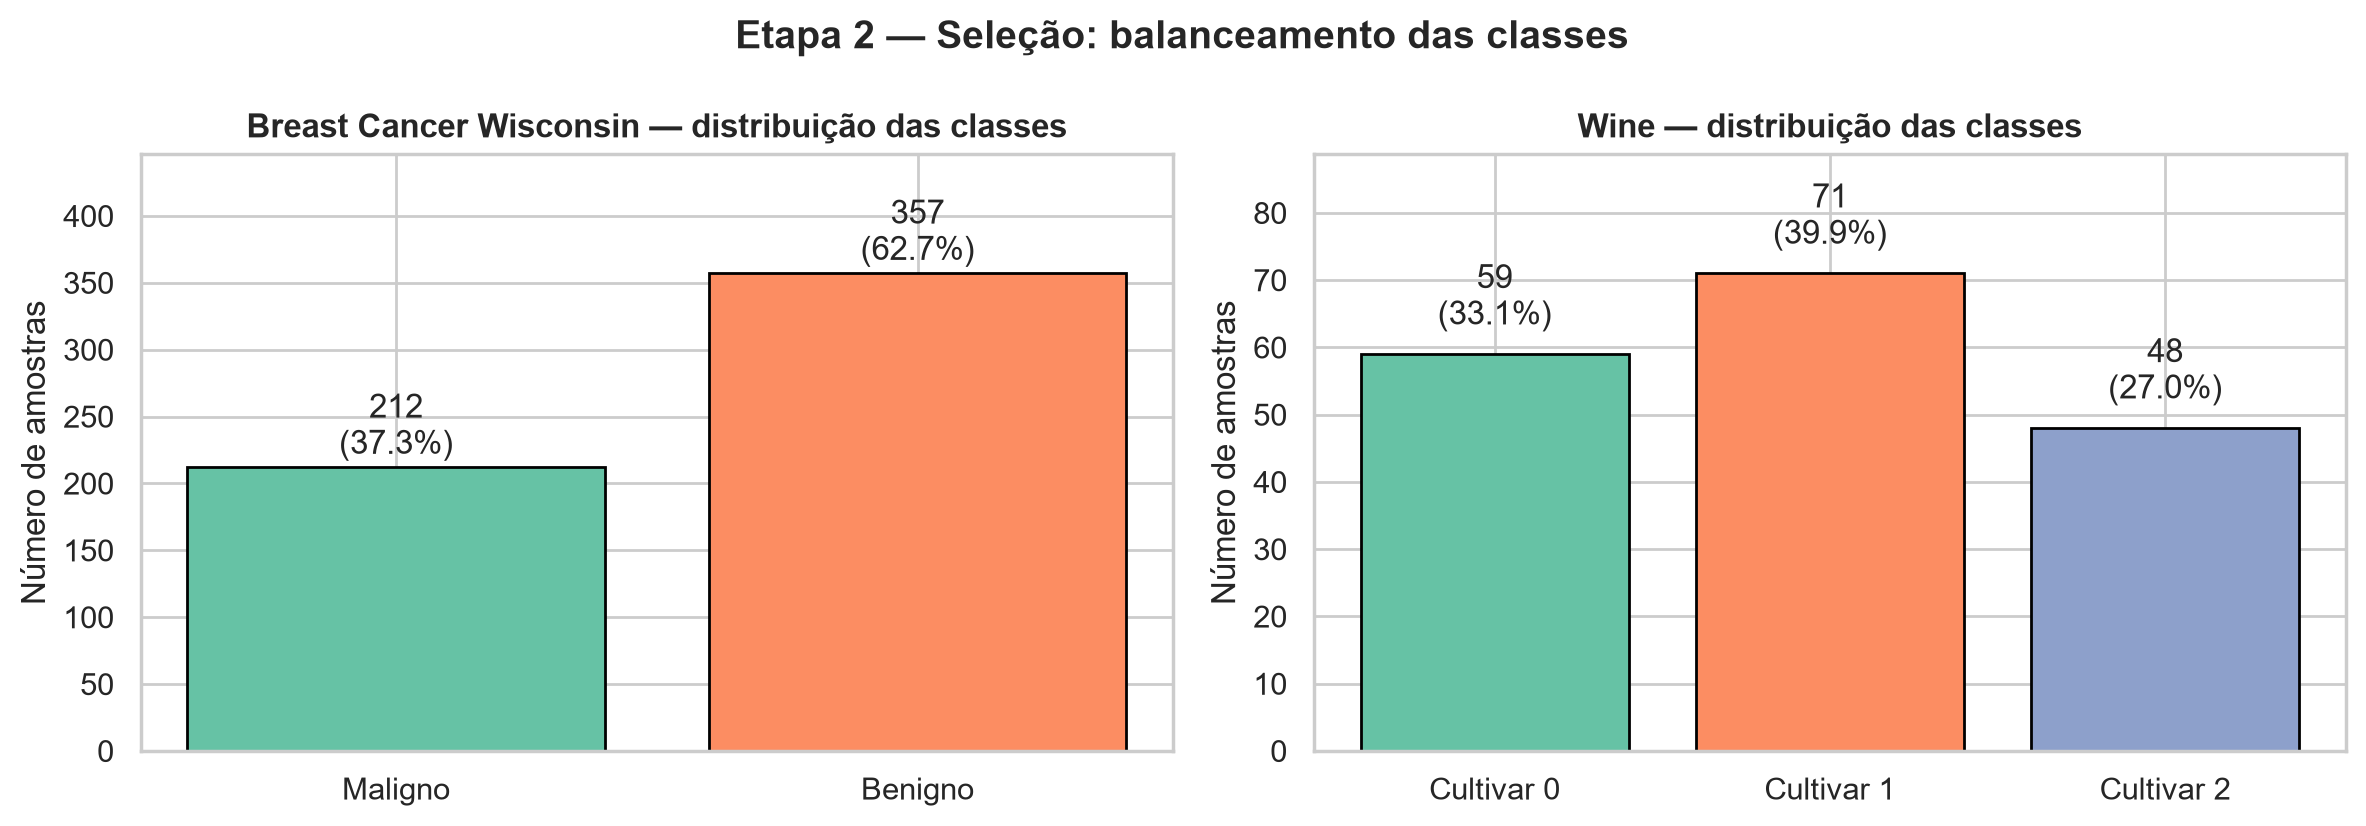
\includegraphics[width=\textwidth, keepaspectratio]{figuras/E2_distribuicao_classes.png}
    \caption{Distribuição das classes nos conjuntos Breast Cancer Wisconsin e Wine.}
    \label{fig:distribuicao_classes}
\end{figure}

\section{ETAPA 3: PRÉ-PROCESSAMENTO}

\subsection{QUALIDADE DOS DADOS}

Não foram encontrados valores ausentes, linhas duplicadas, atributos constantes nem valores negativos, portanto nenhuma limpeza de registros foi necessária. Por outro lado, a razão entre o maior e o menor desvio padrão dos atributos é de 215.170,7 no Breast Cancer (por exemplo, \texttt{area} contra \texttt{smoothness}) e de 2.530,3 no Wine (\texttt{proline} contra \texttt{hue}). Os atributos estão, portanto, em escalas muito diferentes, o que torna a padronização obrigatória para os métodos baseados em distância (KNN, grafos de vizinhança, K-Médias e DBSCAN).

\subsection{\textit{OUTLIERS}}

Pelo critério de Tukey (1,5 $\times$ IQR), 30,1\% das amostras do Breast Cancer possuem pelo menos um atributo \textit{outlier}, e elas se concentram fortemente na classe maligna (53,8\% dos malignos, contra 16,0\% dos benignos). Tumores malignos têm núcleos maiores e mais irregulares, de modo que valores extremos de área, raio e concavidade são \textbf{informação diagnóstica, e não ruído}. Removê-los apagaria justamente os casos mais típicos de malignidade. No Wine, apenas 9,6\% das amostras possuem algum \textit{outlier}. \textbf{Decisão: os \textit{outliers} foram mantidos} nos dois conjuntos.

\subsection{RELEVÂNCIA E SEPARABILIDADE DOS ATRIBUTOS}

A relevância de cada atributo foi medida pela estatística F da ANOVA e pela informação mútua com a classe. As duas medidas produzem rankings muito parecidos (correlação de Spearman de 0,957 no Breast Cancer e 0,951 no Wine). Os atributos mais relevantes são \texttt{worst concave points}, \texttt{worst perimeter} e \texttt{mean concave points} no Breast Cancer, e \texttt{flavanoids}, \texttt{proline} e \texttt{od280/od315} no Wine.

As Figuras \ref{fig:boxplots_bc} e \ref{fig:boxplots_wine} mostram a distribuição, por classe, de três atributos fortemente discriminativos de cada base, os mesmos usados na apresentação. No Breast Cancer, há um intervalo vazio entre o 3º quartil dos benignos e o 1º quartil dos malignos (``zona de segurança''): 13,4 a 15,1 para \texttt{mean radius}, 0,033 a 0,065 para \texttt{mean concave points} e 86 a 99 para \texttt{mean perimeter}. Quanto maior essa distância, maior a margem para o modelo acertar sem confundir os diagnósticos. Por outro lado, os bigodes das duas classes se cruzam, o que caracteriza casos ambíguos e o risco de falsos negativos quando se usa uma única variável. O uso conjunto dos 30 atributos atenua essa ambiguidade.

\begin{figure}[htbp]
    \centering
    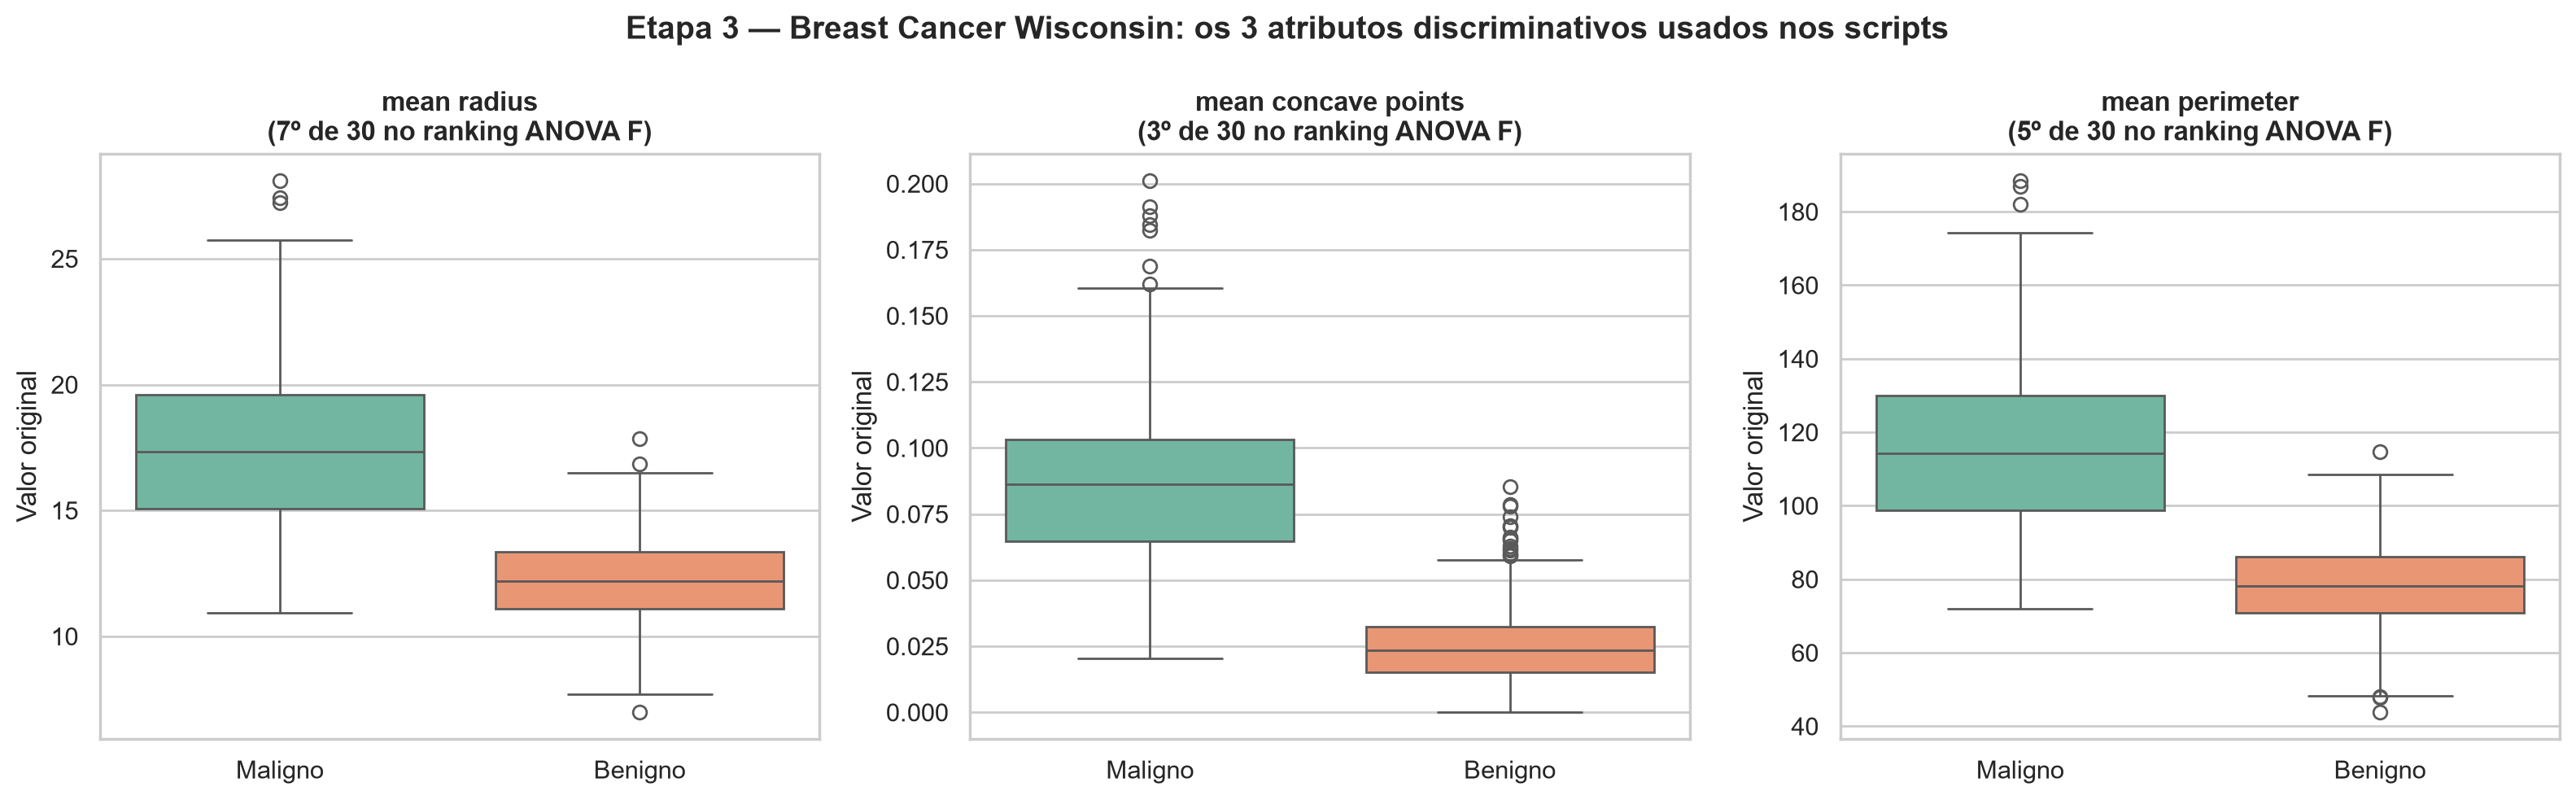
\includegraphics[width=\textwidth, keepaspectratio]{figuras/E3_breast_cancer_atributos_scripts.png}
    \caption{Breast Cancer Wisconsin: distribuição de \texttt{mean radius}, \texttt{mean concave points} e \texttt{mean perimeter} por classe. Os títulos indicam a posição de cada atributo no ranking da ANOVA.}
    \label{fig:boxplots_bc}
\end{figure}

No Wine, \texttt{flavanoids} separa bem as três cultivares, com intervalos vazios de 2,48 a 2,68 (entre as cultivares 1 e 0) e de 0,92 a 1,60 (entre as cultivares 2 e 1). Já \texttt{color\_intensity} e \texttt{alcohol} separam bem a cultivar 1 das demais (intervalos de 3,40 a 4,55 e de 12,52 a 12,80, respectivamente), mas apresentam sobreposição entre as cultivares 0 e 2. O problema multiclasse exige, portanto, a combinação dos atributos, com \texttt{flavanoids} atuando como critério de desempate.

\begin{figure}[htbp]
    \centering
    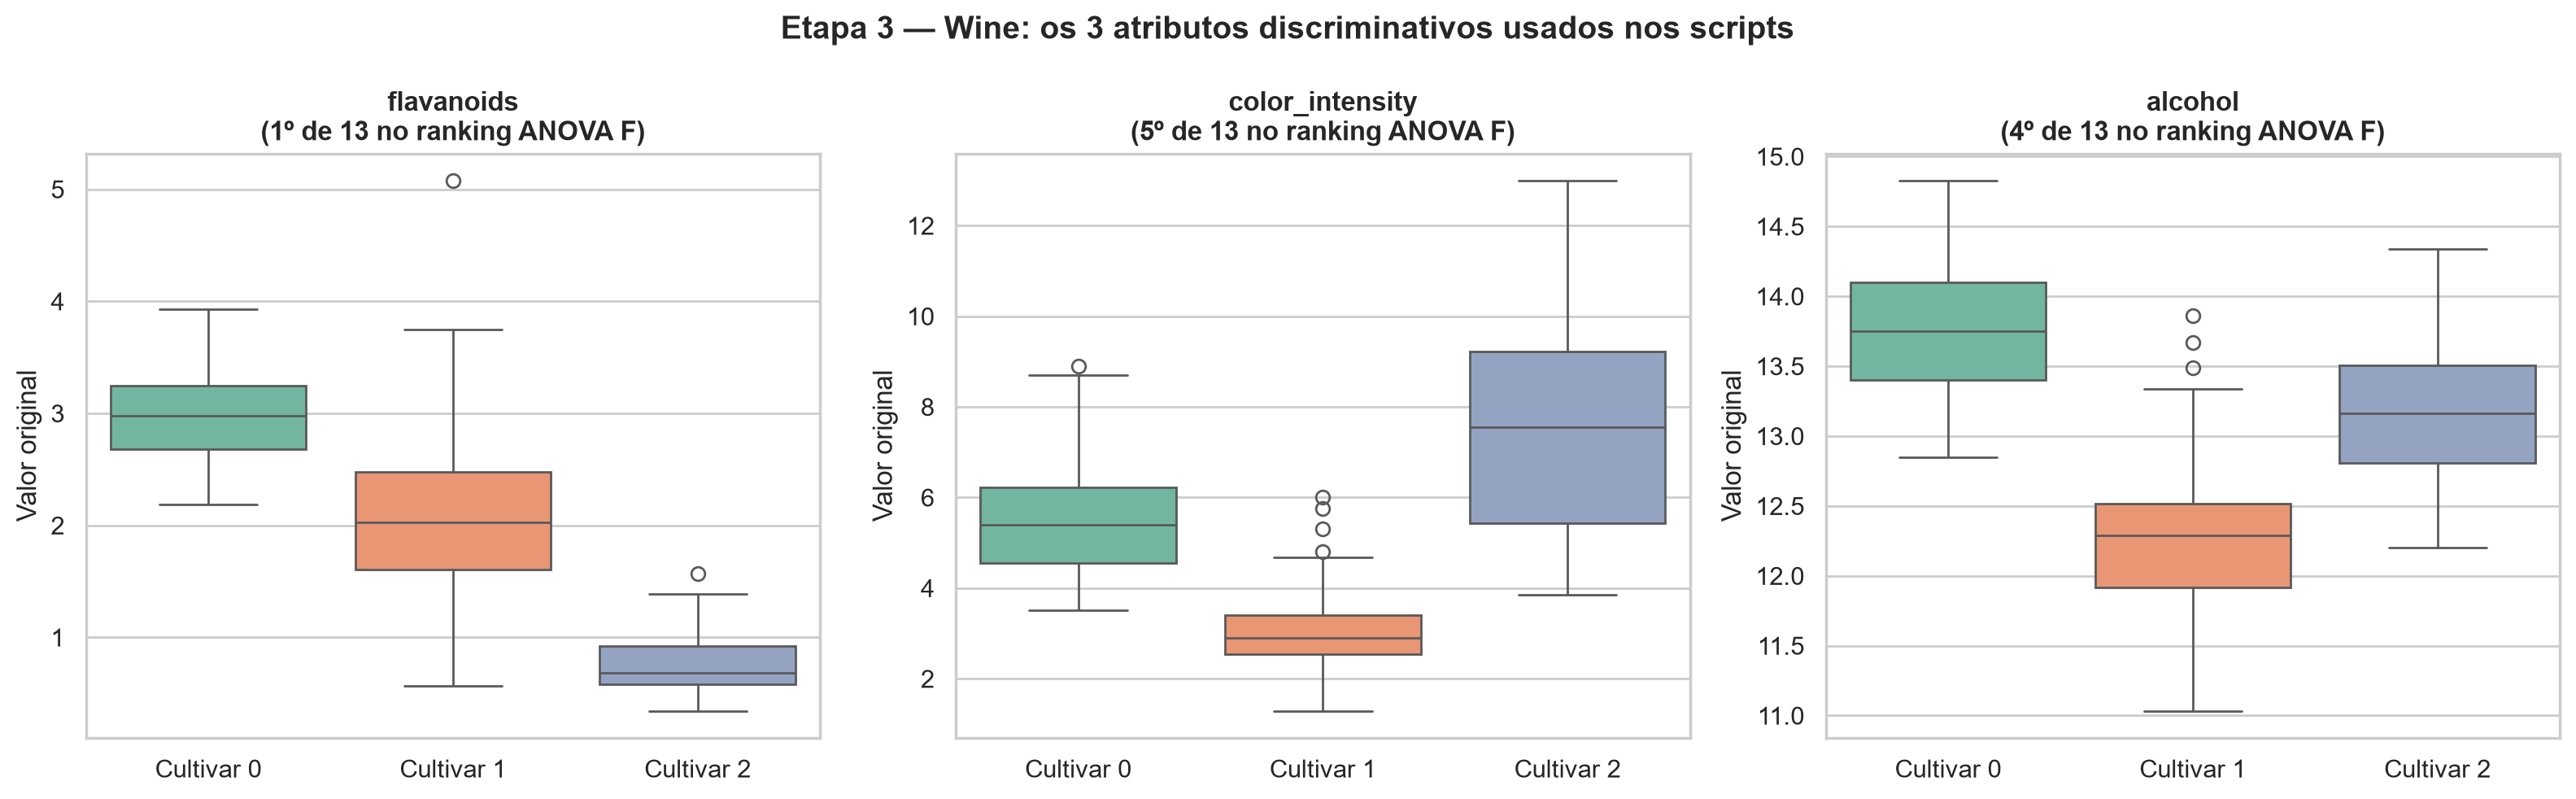
\includegraphics[width=\textwidth, keepaspectratio]{figuras/E3_wine_atributos_scripts.png}
    \caption{Wine: distribuição de \texttt{flavanoids}, \texttt{color\_intensity} e \texttt{alcohol} por cultivar.}
    \label{fig:boxplots_wine}
\end{figure}

\subsection{CORRELAÇÃO ENTRE ATRIBUTOS}

O Breast Cancer apresenta forte redundância: 21 pares de atributos têm correlação $|r| > 0{,}9$. Raio, perímetro e área carregam praticamente a mesma informação ($r \approx 0{,}99$). No Wine, nenhum par ultrapassa esse limite.

\subsection{PARTIÇÃO TREINO/TESTE E PADRONIZAÇÃO}

Antes de qualquer ajuste estatístico, 25\% de cada conjunto foram separados, de forma estratificada, para teste. O conjunto de teste ficou isolado e foi usado apenas para medir o desempenho final. Toda decisão que alimenta os modelos (padronização, PCA e hiperparâmetros) foi ajustada somente no treino.

Para escolher o escalonamento, foi comparado, por validação cruzada estratificada de 5 \textit{folds} no treino, o efeito de quatro opções no KNN ($k = 5$) e na Regressão Logística (Figura \ref{fig:padronizacao} e Tabela \ref{tab:padronizacao}). O escalonador foi ajustado dentro do \textit{pipeline} a cada \textit{fold}, sem vazamento de informação.

\begin{table}[htbp]
\centering
\caption{F1-macro médio (validação cruzada de 5 \textit{folds}) para diferentes escalonamentos.}
\label{tab:padronizacao}
\footnotesize
\begin{tabular}{llcccc}
\toprule
\textbf{Base} & \textbf{Modelo} & \textbf{Nenhum} & \textbf{Standard} & \textbf{MinMax} & \textbf{Robust} \\
\midrule
\multirow{2}{*}{Breast Cancer} & KNN ($k=5$) & 0,934 & 0,964 & 0,967 & 0,959 \\
 & Reg. Logística & 0,942 & 0,977 & 0,969 & 0,975 \\
\midrule
\multirow{2}{*}{Wine} & KNN ($k=5$) & 0,632 & 0,956 & 0,970 & 0,942 \\
 & Reg. Logística & 0,971 & 0,978 & 0,985 & 0,985 \\
\bottomrule
\end{tabular}
\end{table}

\begin{figure}[htbp]
    \centering
    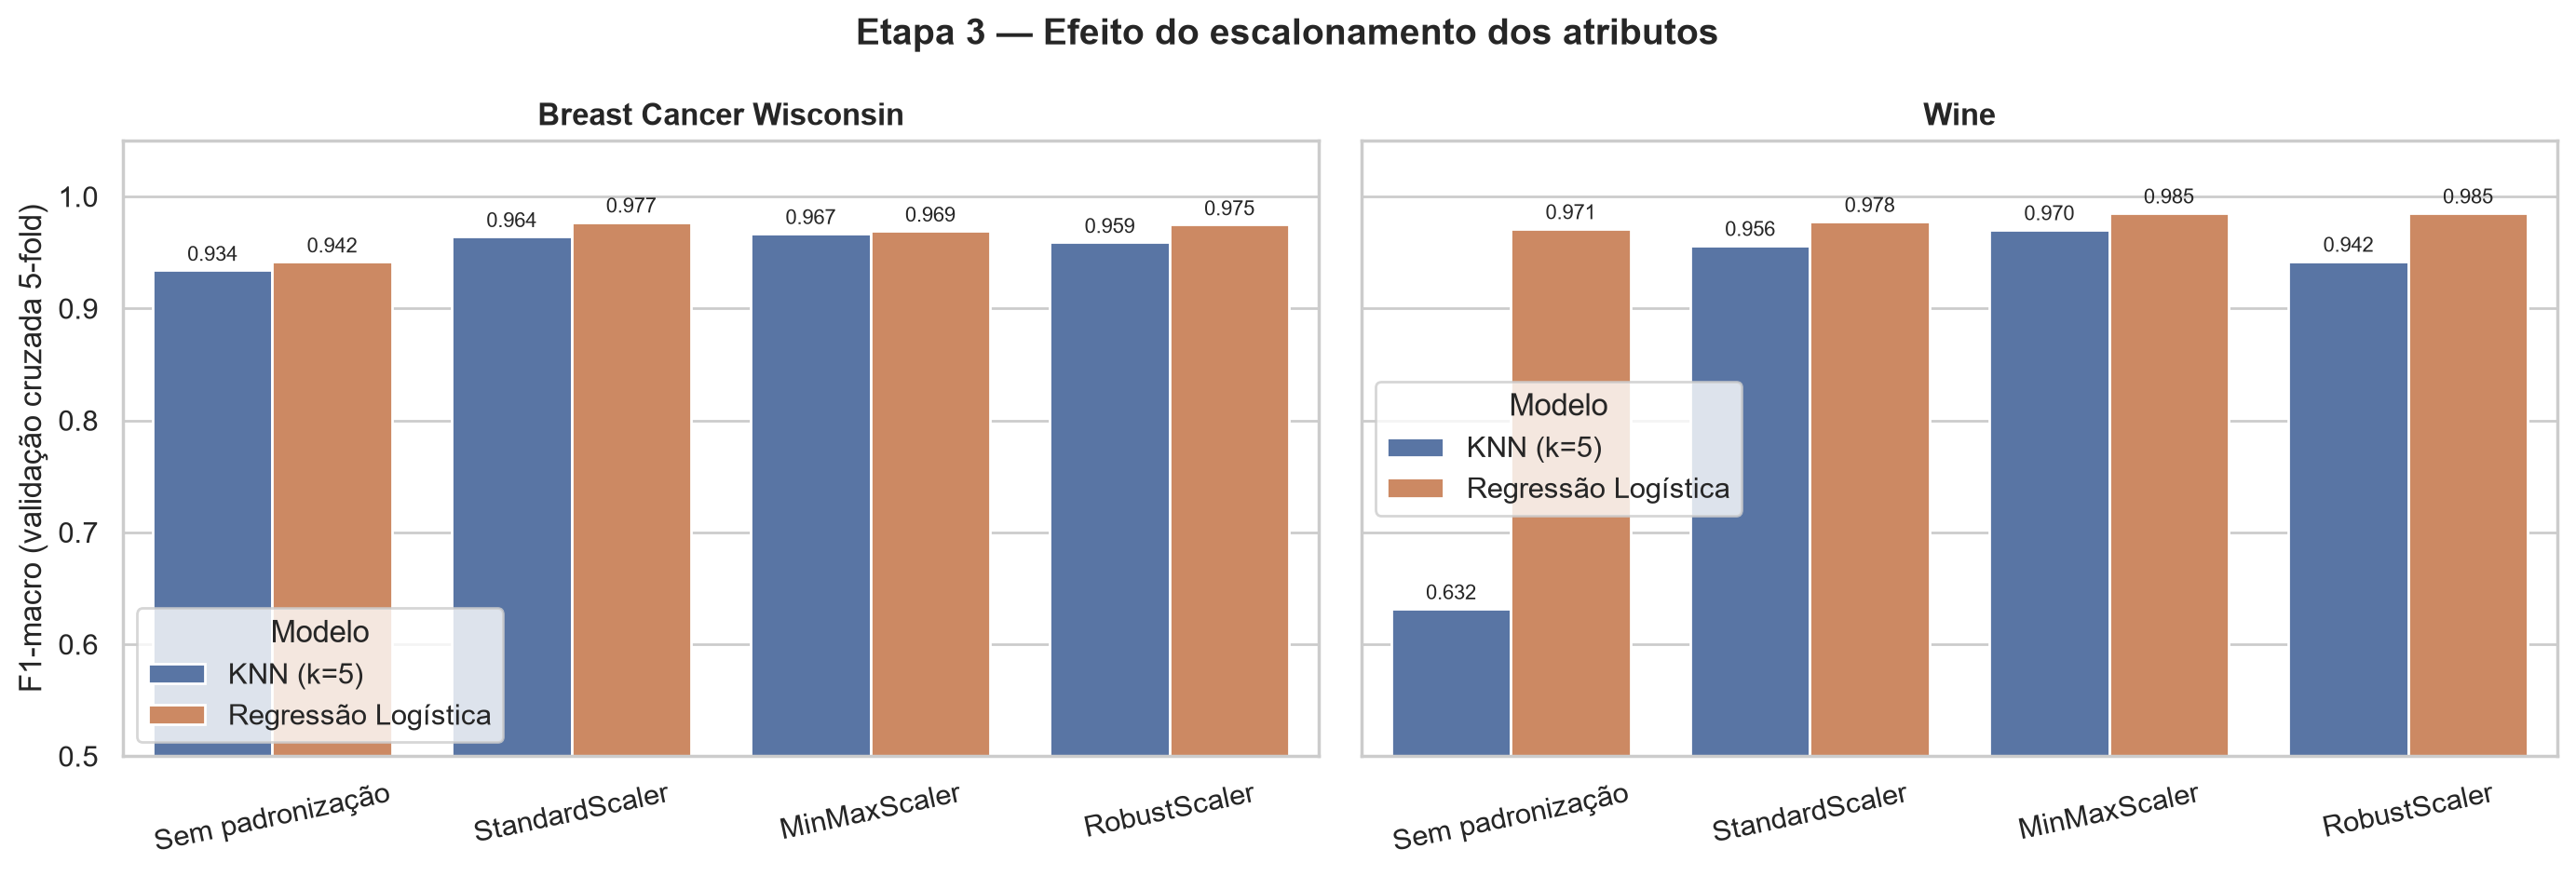
\includegraphics[width=\textwidth, keepaspectratio]{figuras/E3_efeito_padronizacao.png}
    \caption{Efeito do escalonamento no F1-macro do KNN e da Regressão Logística (validação cruzada no treino).}
    \label{fig:padronizacao}
\end{figure}

O escalonamento é decisivo para o KNN no Wine: o F1 sobe de 0,632, sem padronização, para 0,956 com o \texttt{StandardScaler}. Sem escalonamento, a distância euclidiana é dominada por \texttt{proline} (desvio padrão $\approx$ 315) e \texttt{magnesium} ($\approx$ 14). Entre os escalonadores, as diferenças ficam dentro de um desvio padrão da validação cruzada. \textbf{Decisão: \texttt{StandardScaler}}, pois não perde de forma consistente para os demais e deixa todos os atributos com média zero e variância unitária. Com isso, o PCA da Etapa 4 equivale ao PCA da matriz de correlação, e nenhuma unidade de medida domina as componentes.

\section{ETAPA 4: TRANSFORMAÇÃO}

Foram investigadas duas representações de baixa dimensão, ambas não supervisionadas e ajustadas apenas no treino padronizado: o PCA, linear, e os \textit{Laplacian Eigenmaps}, não lineares e baseados em grafo de vizinhança. A Tabela \ref{tab:pca} resume a variância explicada pelo PCA.

\begin{table}[htbp]
\centering
\caption{Variância explicada pelo PCA no treino padronizado.}
\label{tab:pca}
\footnotesize
\begin{tabular}{lcccccc}
\toprule
\textbf{Base} & \textbf{PC1} & \textbf{PC2} & \textbf{PC1+PC2} & \textbf{CPs p/ 90\%} & \textbf{CPs p/ 95\%} & \textbf{Dim. original} \\
\midrule
Breast Cancer & 43,9\% & 19,5\% & 63,4\% & 7 & 10 & 30 \\
Wine & 35,7\% & 19,2\% & 55,0\% & 8 & 10 & 13 \\
\bottomrule
\end{tabular}
\end{table}

A redundância observada no Breast Cancer faz com que a PC1 sozinha concentre 43,9\% da variância. No biplot da Figura \ref{fig:biplot_bc}, a PC1 aponta na direção dos atributos de \textbf{tamanho} (raio, perímetro e área), e os tumores malignos ocupam a região de PC1 alto. A PC2 é dominada pela dimensão fractal, quase ortogonal ao diagnóstico. No Wine, a variância é mais distribuída entre as componentes.

\begin{figure}[htbp]
    \centering
    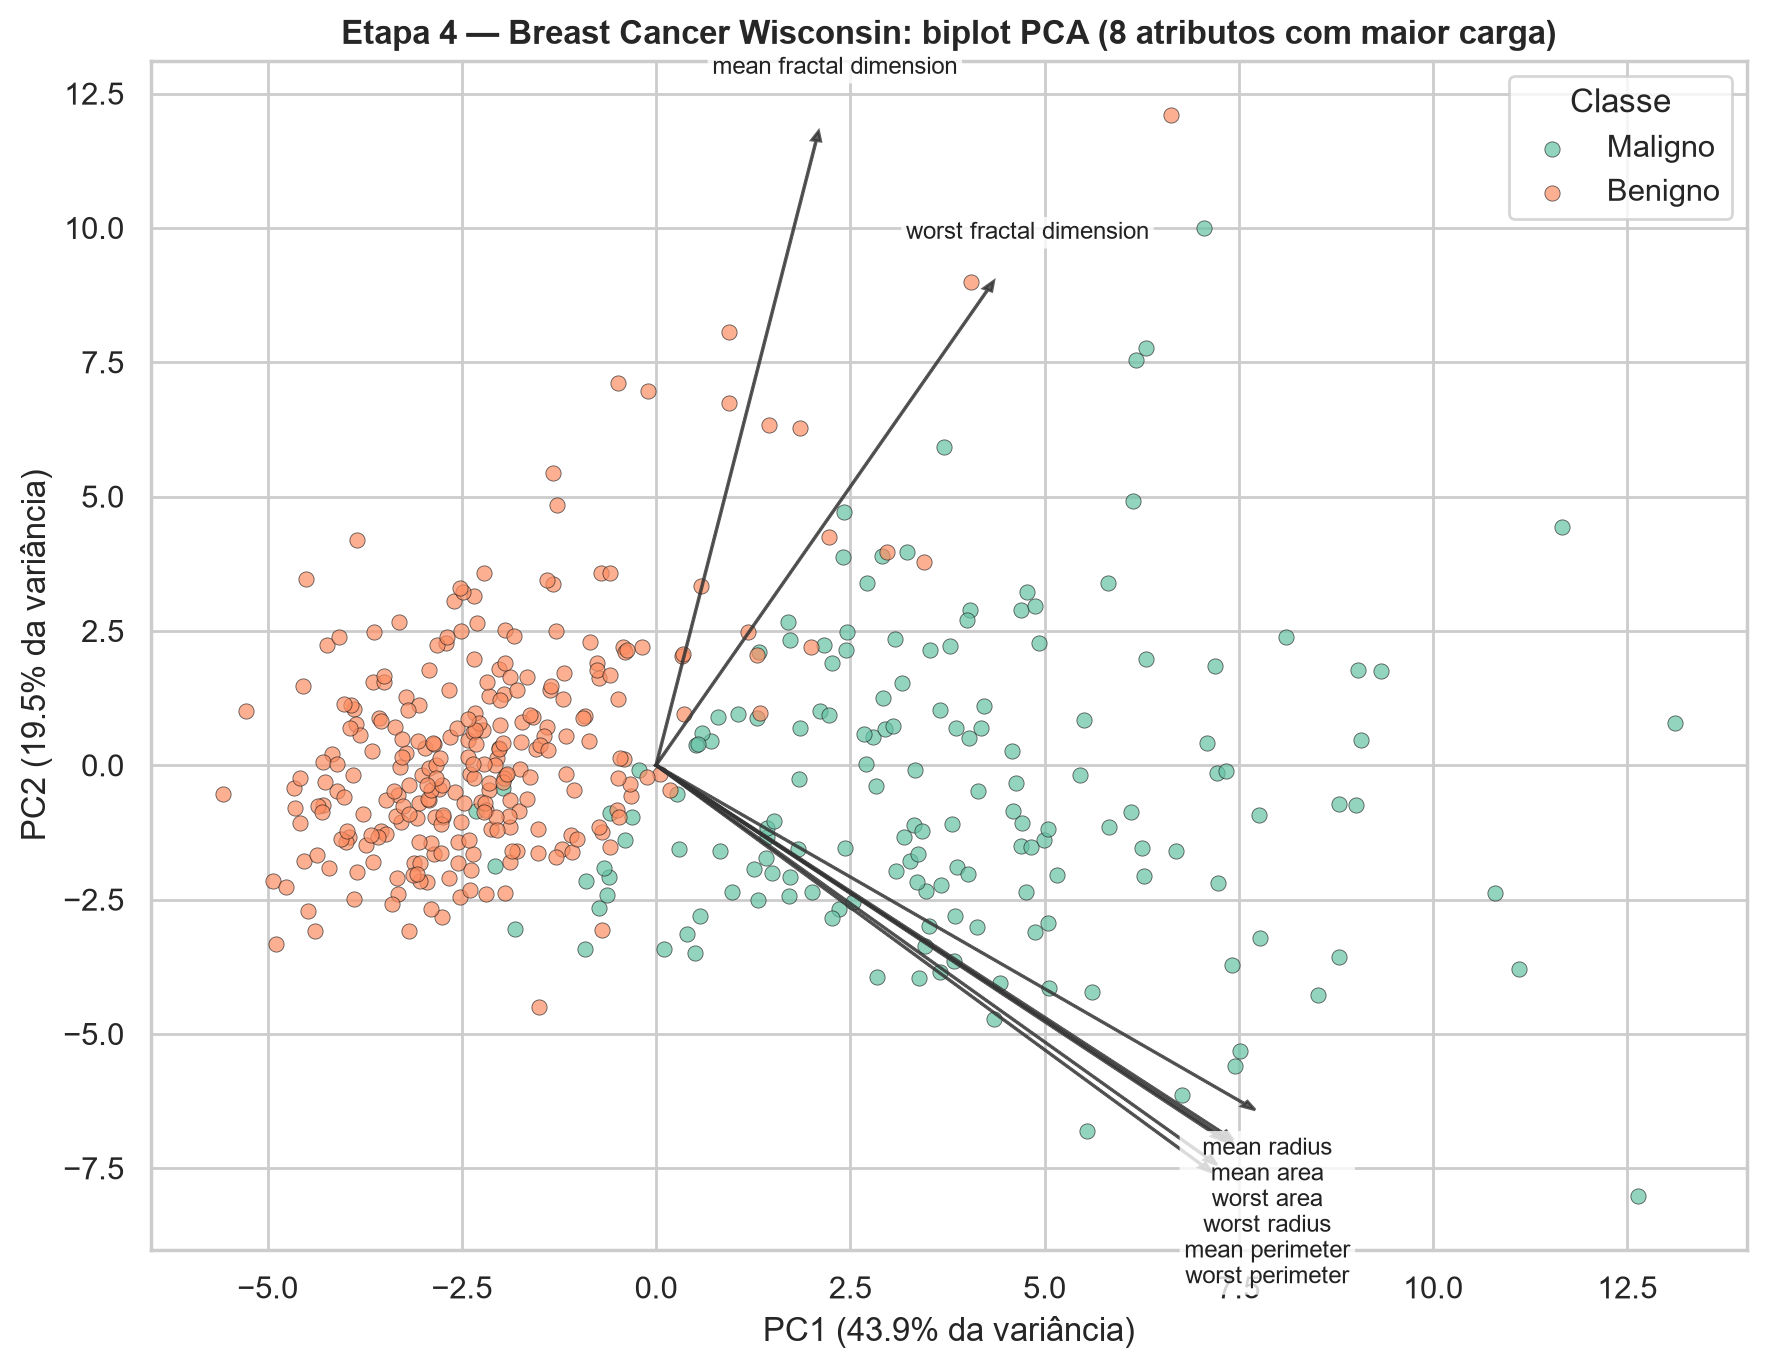
\includegraphics[width=0.85\textwidth, keepaspectratio]{figuras/E4_breast_cancer_pca_biplot.png}
    \caption{Breast Cancer Wisconsin: projeção PCA 2D do treino e cargas (\textit{loadings}) dos atributos mais relevantes.}
    \label{fig:biplot_bc}
\end{figure}

Para medir quanto da separabilidade das classes cada representação preserva, foram calculadas a silhueta das classes reais e o F1-macro de um KNN ($k = 5$) em validação cruzada (Figura \ref{fig:separabilidade}). No Wine, o KNN no PCA 2D (F1 = 0,978) chega a superar o espaço completo (0,963), pois as dimensões descartadas carregam mais ruído do que sinal. No Breast Cancer, a perda é pequena (de 0,962 para 0,932). A silhueta das classes reais aumenta nas projeções 2D (no Wine, de 0,281 para 0,542 no PCA e 0,767 nos \textit{Laplacian Eigenmaps}). Isso indica que, no espaço completo, as distâncias são ``diluídas'' por atributos pouco discriminativos, efeito que prejudica os métodos baseados em densidade. Os grupos muito compactos obtidos pelos \textit{Laplacian Eigenmaps} no Wine indicam que a hipótese de \textit{cluster} vale bem nessa base.

\begin{figure}[htbp]
    \centering
    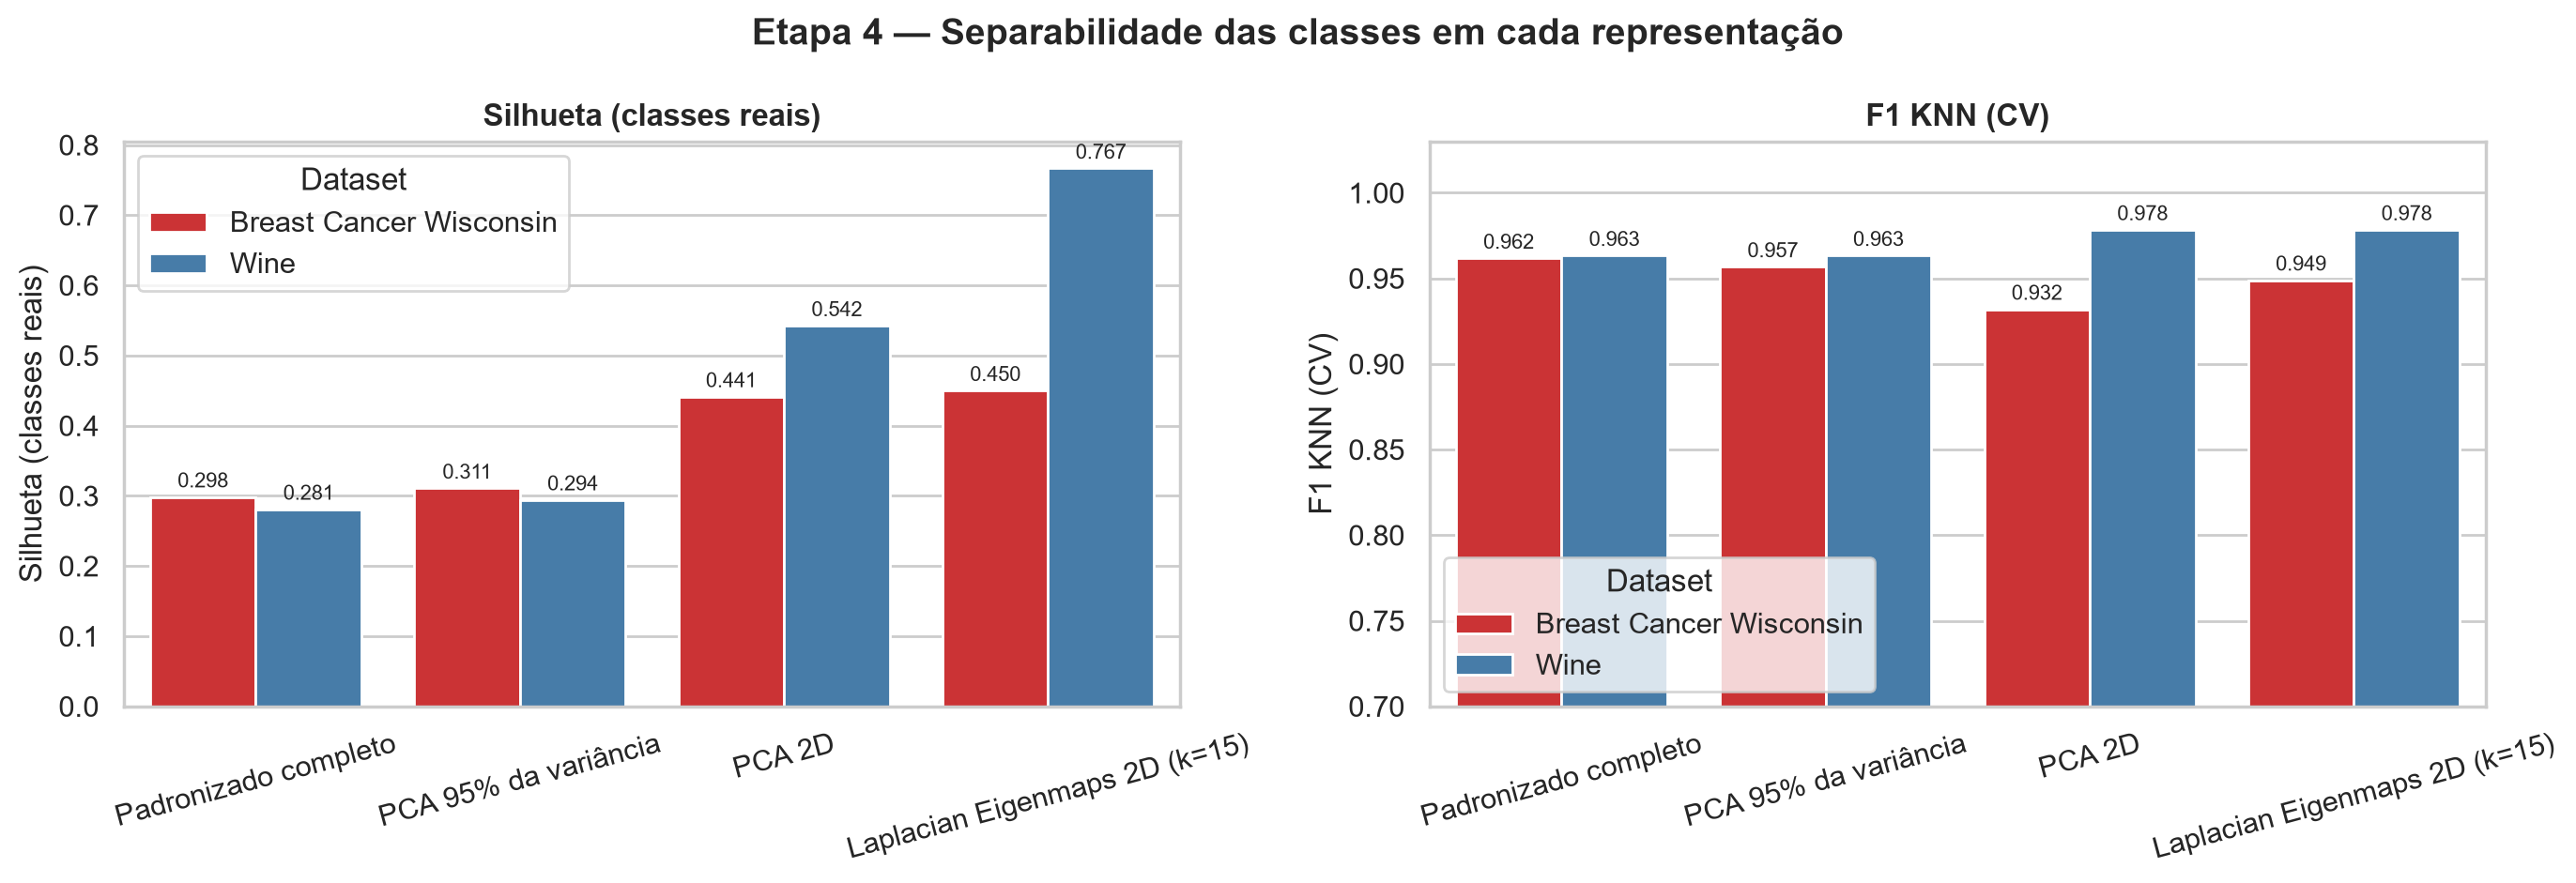
\includegraphics[width=\textwidth, keepaspectratio]{figuras/E4_separabilidade_representacoes.png}
    \caption{Separabilidade das classes em cada representação: silhueta das classes reais e F1-macro do KNN em validação cruzada.}
    \label{fig:separabilidade}
\end{figure}

\textbf{Decisão:} os classificadores e os agrupamentos trabalham no \textbf{espaço padronizado completo}, sem perda de informação. As projeções 2D são usadas apenas para visualização.

\section{PROTOCOLO EXPERIMENTAL DA ETAPA 5}

O agrupamento foi aplicado ao treino padronizado \textbf{sem nenhum rótulo}. Os rótulos verdadeiros foram usados somente para avaliar os agrupamentos.

Na classificação semi-supervisionada, para cada taxa e repetição, uma fração estratificada dos pontos de treino manteve o rótulo e os demais foram marcados como não rotulados. Em cada repetição, todos os modelos receberam \textbf{o mesmo} subconjunto rotulado, o que permite comparações pareadas. Os \textit{baselines} foram treinados apenas com os pontos rotulados, enquanto os semi-supervisionados usaram também os não rotulados. A avaliação principal foi feita no conjunto de teste isolado. O sorteio estratificado evita que uma classe inteira fique sem nenhum ponto rotulado; no Wine, em que 5\% do treino correspondem a apenas 7 amostras, foi imposto ainda um mínimo de dois pontos rotulados por cultivar. Os dois \textit{scripts} adotaram protocolos ligeiramente diferentes, resumidos na Tabela \ref{tab:protocolo}.

\begin{table}[htbp]
\centering
\caption{Protocolo experimental de cada conjunto de dados.}
\label{tab:protocolo}
\footnotesize
\begin{tabular}{p{3.0cm} p{5.6cm} p{5.6cm}}
\toprule
\textbf{Item} & \textbf{Breast Cancer Wisconsin} & \textbf{Wine} \\
\midrule
Taxas de rótulos & 0,05; 0,10; 0,20; 0,30; 0,40; 0,50; 0,60; 0,70 & 0,05; 0,10; 0,20; 0,30; 0,50; 0,70 \\
\addlinespace
Repetições & 5 (sementes 10, 20, 30, 40 e 50) & 10 (sementes 100 a 109) \\
\addlinespace
Sorteio dos rotulados & Estratificado & Estratificado, com no mínimo 2 por classe \\
\addlinespace
\textit{Baselines} & KNN ($k = 5$); Regressão Logística & KNN ($k = \min(5, n_{\text{rot}}/2)$); Regressão Logística \\
\addlinespace
Semi-supervisionados & \textit{Label Spreading} (grafo kNN, $k = 7$); \textit{Self-Training} com RL (limiar 0,75) & \textit{Label Spreading} e \textit{Label Propagation} (RBF, $\gamma = 1/13$); \textit{Self-Training} com RL (limiar 0,80) \\
\addlinespace
K-Médias & $k = 2$, \texttt{n\_init} = 10 & $k = 3$, \texttt{n\_init} = 20 \\
\addlinespace
DBSCAN & \texttt{eps} = 4,5; \texttt{min\_samples} = 5 & \texttt{eps} = 2,3; \texttt{min\_samples} = 4 \\
\bottomrule
\end{tabular}
\end{table}

\chapter[Resultados da Mineração]{RESULTADOS DA MINERAÇÃO}

Este capítulo apresenta os resultados da Etapa 5 do processo KDD. Primeiro é discutido o agrupamento, o caso-limite com 0\% de rótulos, e em seguida a classificação semi-supervisionada com taxas de rotulagem de 5\% a 70\%.

\section{AGRUPAMENTO: O CASO-LIMITE COM 0\% DE RÓTULOS}

\subsection{ESCOLHA DO NÚMERO DE GRUPOS NO K-MÉDIAS}

Para verificar se a estrutura dos dados sugere, por si só, o número de classes, o K-Médias foi executado com $k$ de 2 a 10, registrando a inércia (método do cotovelo) e a silhueta. A silhueta, que não usa rótulos, atinge o máximo exatamente no número real de classes nas duas bases: $k = 2$ no Breast Cancer (silhueta de 0,349) e $k = 3$ no Wine (0,288), como mostra a Figura \ref{fig:kmeans_k_wine} para o Wine.

\begin{figure}[htbp]
    \centering
    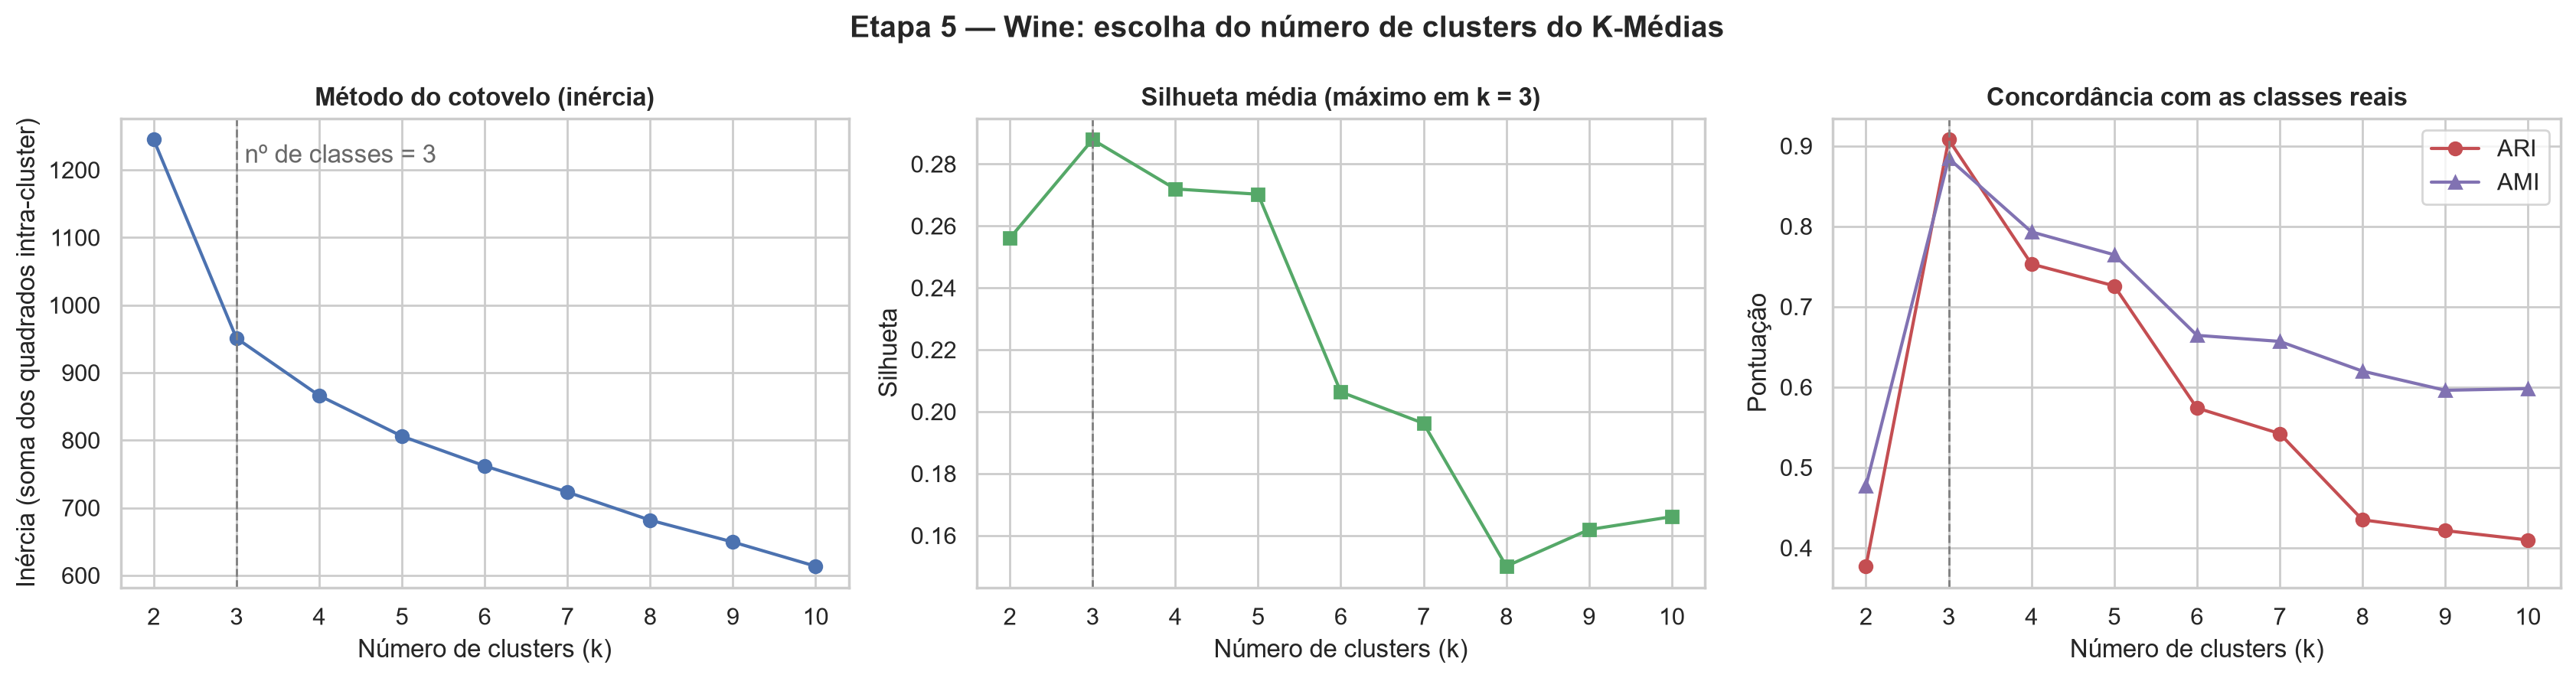
\includegraphics[width=\textwidth, keepaspectratio]{figuras/E5_wine_kmeans_escolha_k.png}
    \caption{Wine: inércia, silhueta e concordância com as classes reais (ARI e AMI) do K-Médias em função de $k$.}
    \label{fig:kmeans_k_wine}
\end{figure}

\subsection{K-MÉDIAS E DBSCAN}

A Tabela \ref{tab:agrupamento} resume as métricas de agrupamento com os parâmetros dos \textit{scripts}, e as Figuras \ref{fig:agrupamento_bc} e \ref{fig:agrupamento_wine} mostram os grupos projetados no PCA 2D.

\begin{table}[htbp]
\centering
\caption{Métricas de agrupamento no treino padronizado (0\% rotulado).}
\label{tab:agrupamento}
\begin{tabular}{llccccc}
\toprule
\textbf{Base} & \textbf{Algoritmo} & \textbf{Grupos} & \textbf{Ruído} & \textbf{ARI} & \textbf{NMI} & \textbf{Silhueta} \\
\midrule
\multirow{2}{*}{Breast Cancer} & K-Médias ($k = 2$) & 2 & 0,0\% & 0,672 & 0,555 & 0,349 \\
 & DBSCAN (\texttt{eps} = 4,5) & 1 & 6,1\% & 0,025 & 0,012 & -- \\
\midrule
\multirow{2}{*}{Wine} & K-Médias ($k = 3$) & 3 & 0,0\% & 0,908 & 0,886 & 0,288 \\
 & DBSCAN (\texttt{eps} = 2,3) & 4 & 22,6\% & 0,602 & 0,660 & 0,253 \\
\bottomrule
\end{tabular}
\end{table}

\begin{figure}[htbp]
    \centering
    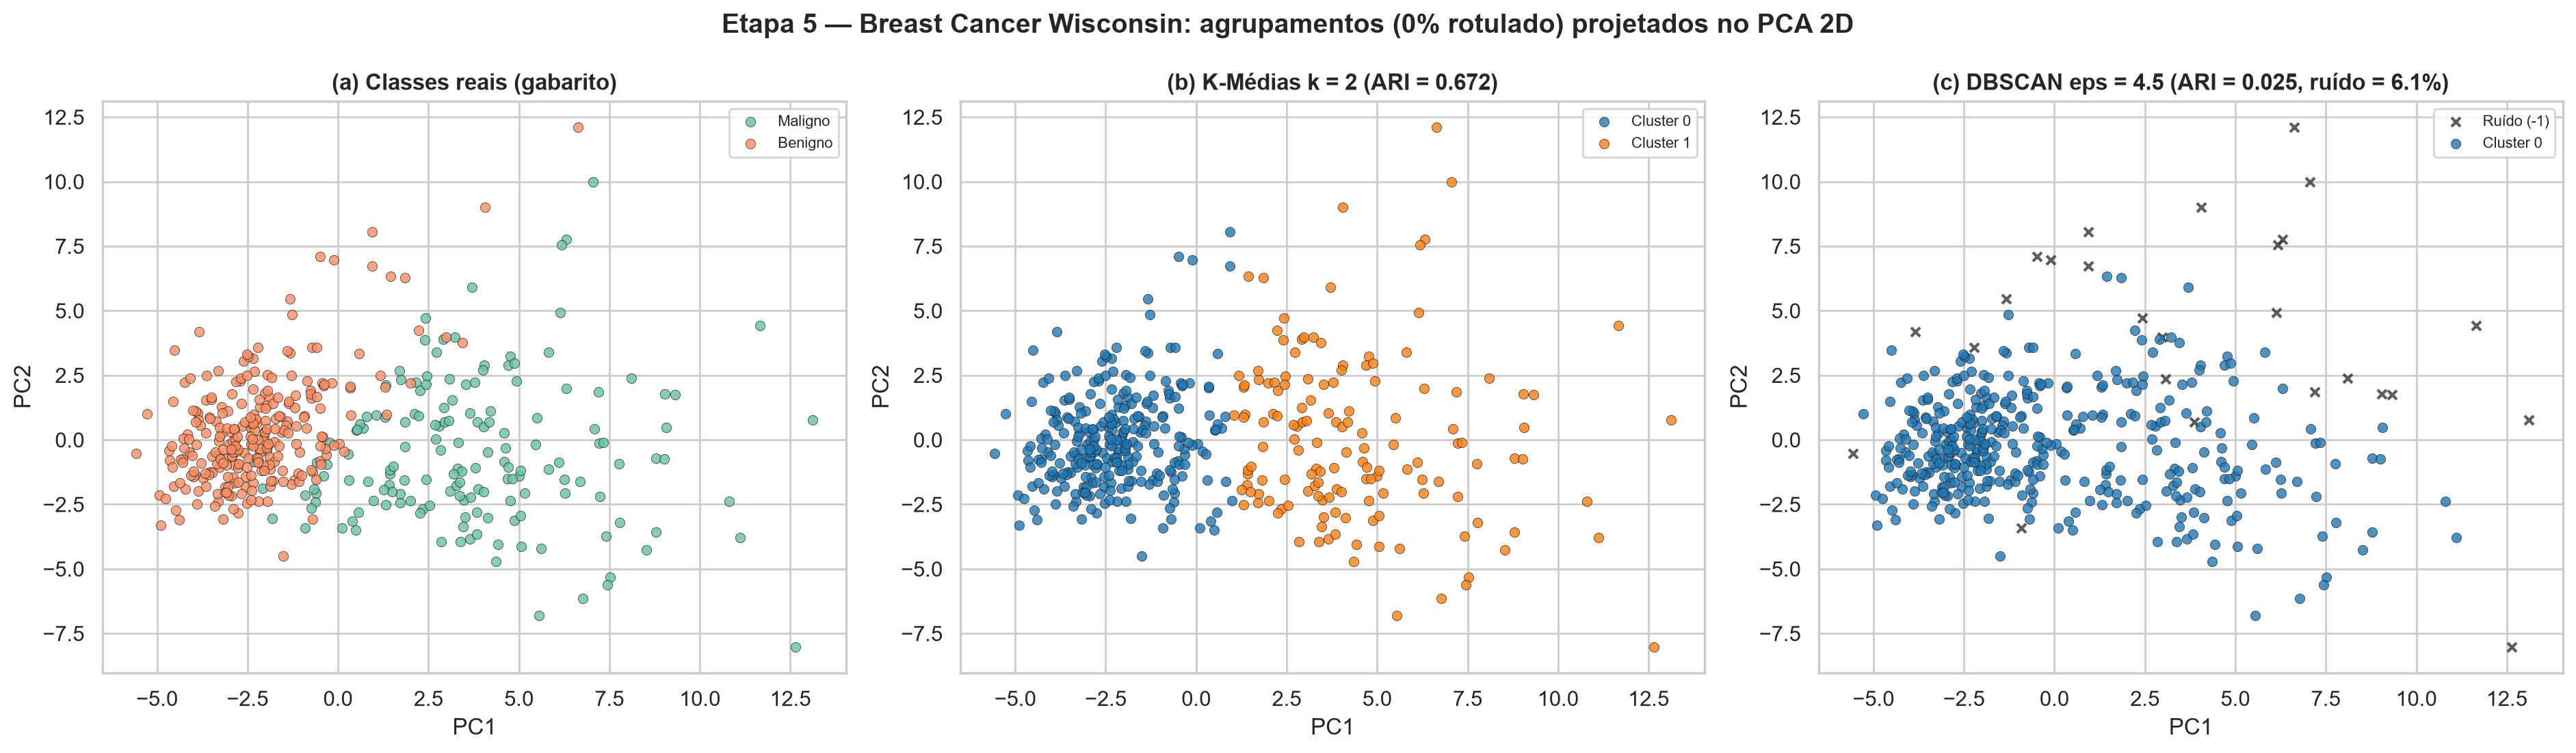
\includegraphics[width=\textwidth, keepaspectratio]{figuras/E5_breast_cancer_agrupamentos_pca.png}
    \caption{Breast Cancer Wisconsin: (a) classes reais, (b) K-Médias e (c) DBSCAN, projetados no PCA 2D.}
    \label{fig:agrupamento_bc}
\end{figure}

No Breast Cancer, os casos benignos formam um grupo compacto, enquanto os malignos se dispersam ao longo da PC1. O K-Médias separa os grupos aproximadamente na mesma fronteira das classes reais (ARI = 0,672). O DBSCAN, por sua vez, une as duas classes em uma massa única e marca como ruído os pontos mais distantes, que são justamente tumores malignos atípicos. O valor de \texttt{eps} do \textit{script} fica próximo ao ``joelho'' da curva de k-distâncias ($\approx$ 4,29). Em uma varredura de 160 combinações de \texttt{eps} e \texttt{min\_samples}, apenas 5 formaram dois ou mais grupos: não existe um ``vale de densidade'' entre benignos e malignos. O melhor ARI da varredura (0,400) foi obtido com um único grupo e 48\% de ruído, ou seja, o DBSCAN só consegue isolar parte da classe maligna como ruído em torno de um núcleo denso. Esse comportamento é coerente com a análise de \textit{outliers} da Etapa 3.

\begin{figure}[htbp]
    \centering
    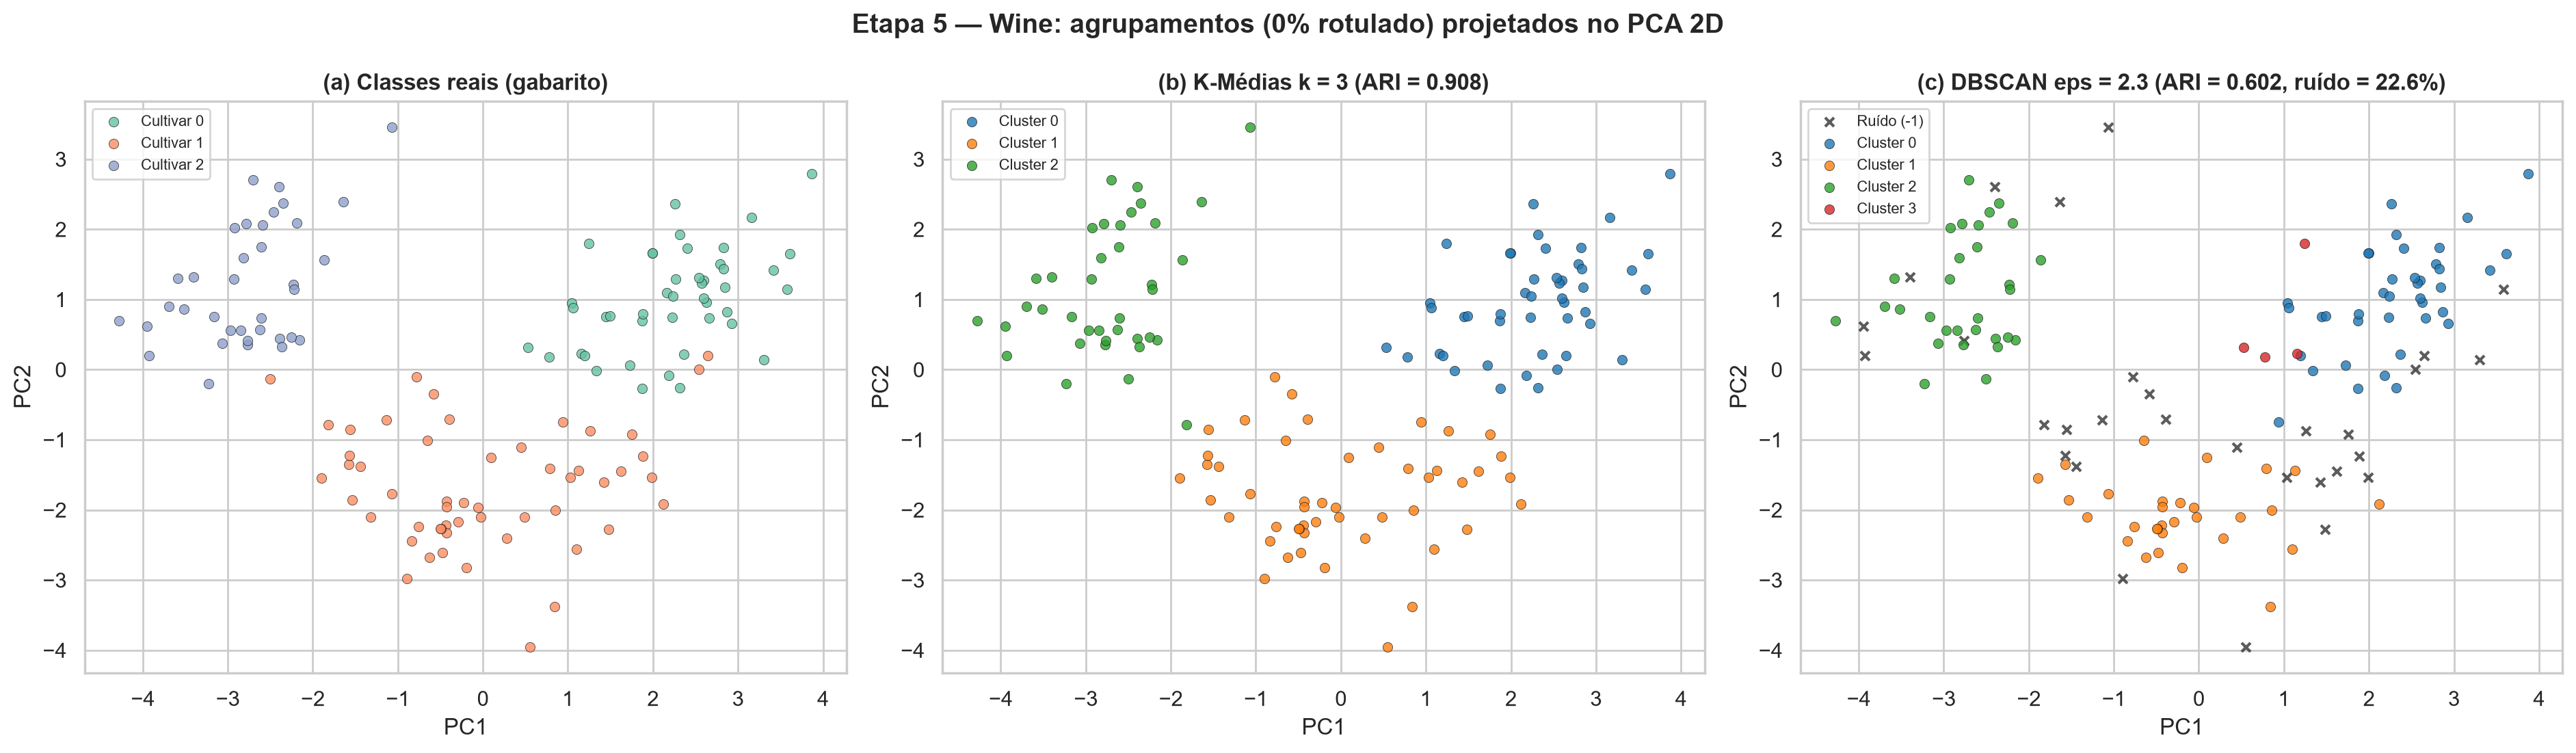
\includegraphics[width=\textwidth, keepaspectratio]{figuras/E5_wine_agrupamentos_pca.png}
    \caption{Wine: (a) classes reais, (b) K-Médias e (c) DBSCAN, projetados no PCA 2D.}
    \label{fig:agrupamento_wine}
\end{figure}

No Wine, as três cultivares formam grupos distintos, com mistura apenas nas faixas de transição, e o K-Médias praticamente reproduz as classes sem nenhum rótulo (ARI = 0,908). O DBSCAN fragmenta a estrutura em quatro grupos e descarta 22,6\% das amostras como ruído, concentrado nas fronteiras entre as cultivares (ARI = 0,602). Esse é o melhor ARI da varredura, mas depende de ajuste fino: com \texttt{min\_samples} = 4, apenas a faixa estreita de \texttt{eps} entre 2,2 e 2,4 separa mais de um grupo, e com \texttt{eps} $\geq$ 2,5, incluindo o joelho da curva ($\approx$ 2,73), tudo se torna um único grupo.

\subsection{DO AGRUPAMENTO AO CLASSIFICADOR}

Para colocar o agrupamento na mesma escala dos classificadores, cada grupo do K-Médias foi associado a uma classe pelo algoritmo húngaro \citep{kuhn1955hungarian}, que encontra a associação um-para-um que maximiza os acertos no treino. Em seguida, os pontos de teste foram atribuídos ao centróide mais próximo. Essa referência é otimista, pois a associação usa os rótulos do treino, mas mostra quanto da estrutura das classes o agrupamento captura sem supervisão: os grupos do K-Médias classificam corretamente \textbf{92,3\%} das amostras de teste no Breast Cancer (F1 = 0,916) e \textbf{95,6\%} no Wine (F1 = 0,956).

Em síntese, após a padronização as classes formam grupos aproximadamente convexos, mas encostados uns nos outros, sem regiões vazias entre elas. Isso favorece o K-Médias e prejudica o DBSCAN. O sucesso do agrupamento no Wine antecipa que os dados não rotulados devem ajudar mais nessa base do que no Breast Cancer.

\section{CLASSIFICAÇÃO SEMI-SUPERVISIONADA}

\subsection{CURVAS DE APRENDIZADO}

As Tabelas \ref{tab:f1_bc} e \ref{tab:f1_wine} e as Figuras \ref{fig:curva_bc} e \ref{fig:curva_wine} apresentam o F1-macro no conjunto de teste em função da taxa de pontos rotulados.

\begin{table}[htbp]
\centering
\caption{Breast Cancer Wisconsin: F1-macro no teste (média $\pm$ desvio padrão em 5 repetições).}
\label{tab:f1_bc}
\footnotesize
\begin{tabular}{ccccc}
\toprule
\textbf{Taxa} & \textbf{KNN} & \textbf{Reg. Logística} & \textbf{Label Spreading} & \textbf{Self-Training LR} \\
\midrule
0,05 & 0,906 $\pm$ 0,014 & 0,926 $\pm$ 0,017 & \textbf{0,936} $\pm$ 0,007 & 0,930 $\pm$ 0,021 \\
0,10 & 0,925 $\pm$ 0,009 & \textbf{0,939} $\pm$ 0,011 & 0,926 $\pm$ 0,011 & 0,936 $\pm$ 0,015 \\
0,20 & 0,942 $\pm$ 0,007 & 0,947 $\pm$ 0,010 & 0,938 $\pm$ 0,014 & \textbf{0,948} $\pm$ 0,007 \\
0,30 & 0,945 $\pm$ 0,017 & \textbf{0,962} $\pm$ 0,012 & 0,944 $\pm$ 0,014 & 0,961 $\pm$ 0,008 \\
0,40 & 0,951 $\pm$ 0,007 & \textbf{0,970} $\pm$ 0,010 & 0,959 $\pm$ 0,012 & 0,965 $\pm$ 0,012 \\
0,50 & 0,956 $\pm$ 0,009 & 0,973 $\pm$ 0,012 & 0,953 $\pm$ 0,014 & \textbf{0,974} $\pm$ 0,009 \\
0,60 & 0,957 $\pm$ 0,007 & \textbf{0,976} $\pm$ 0,006 & 0,956 $\pm$ 0,007 & \textbf{0,976} $\pm$ 0,010 \\
0,70 & 0,964 $\pm$ 0,008 & \textbf{0,982} $\pm$ 0,004 & 0,962 $\pm$ 0,009 & \textbf{0,982} $\pm$ 0,004 \\
\bottomrule
\end{tabular}
\end{table}

\begin{figure}[htbp]
    \centering
    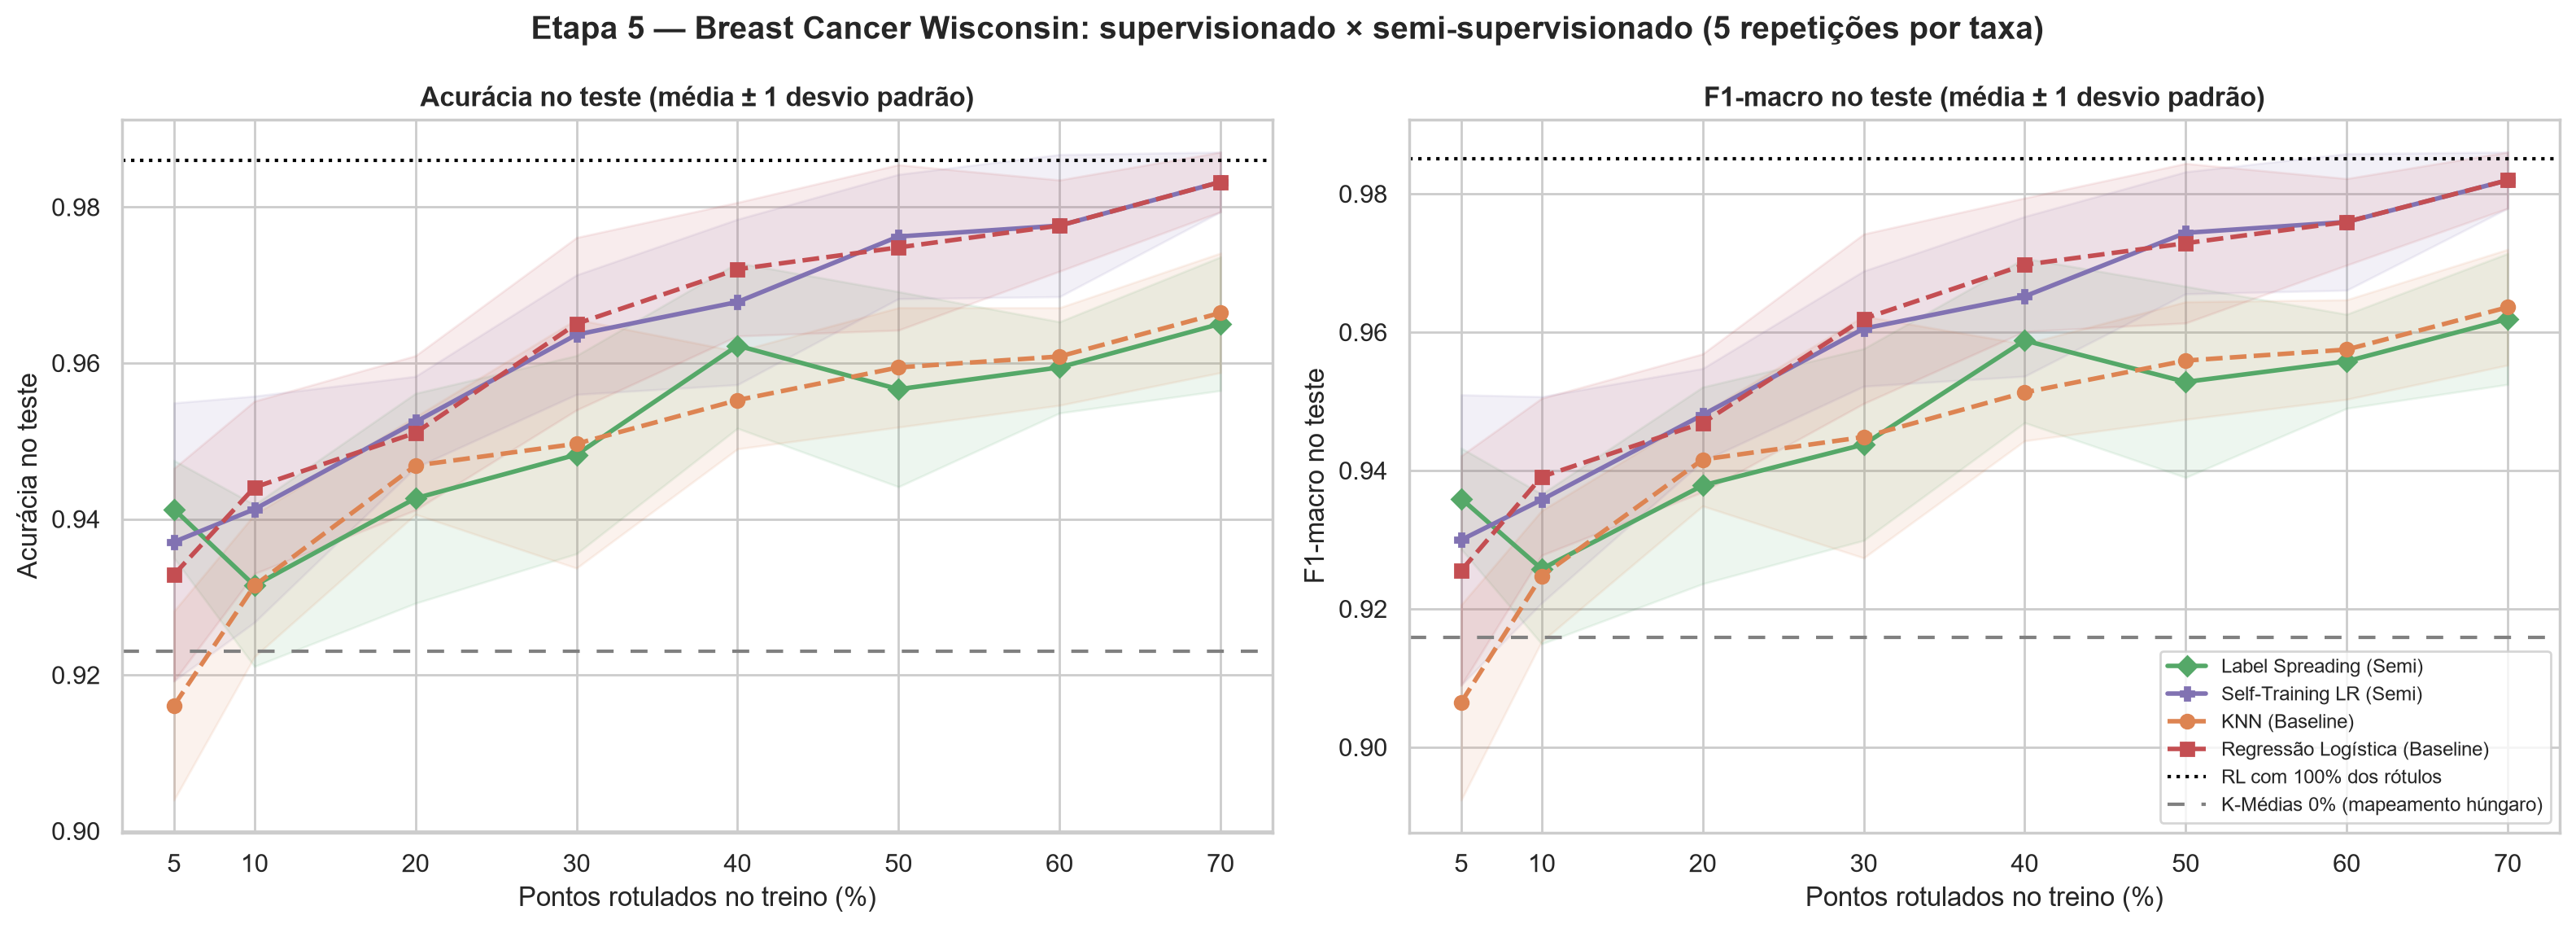
\includegraphics[width=\textwidth, keepaspectratio]{figuras/E5_breast_cancer_curva_aprendizado.png}
    \caption{Breast Cancer Wisconsin: acurácia e F1-macro no teste em função da taxa de rótulos (média $\pm$ 1 desvio padrão).}
    \label{fig:curva_bc}
\end{figure}

No Breast Cancer, com 5\% de rótulos (21 amostras), os métodos semi-\hspace{0pt}supervisionados superam o KNN (de 0,906 para cerca de 0,936), e o \textit{Label Spreading} obtém o maior F1 médio, ligeiramente acima da Regressão Logística (0,936 contra 0,926). As faixas de desvio padrão, no entanto, se sobrepõem, e a partir de 10\% a Regressão Logística já iguala ou supera os métodos semi-supervisionados. Com 70\% dos rótulos, o \textit{Self-Training} e a Regressão Logística produzem exatamente o mesmo F1 (0,982) nas cinco repetições, ou seja, os pseudo-rótulos deixam de alterar as predições no teste. A acurácia média do \textit{Self-Training} considerando todas as taxas de 5\% a 70\% foi de 96,24\%.

\begin{table}[htbp]
\centering
\caption{Wine: F1-macro no teste (média $\pm$ desvio padrão em 10 repetições). Entre parênteses, o número de amostras rotuladas.}
\label{tab:f1_wine}
\footnotesize
\setlength{\tabcolsep}{5pt}
\begin{tabular}{cccccc}
\toprule
\textbf{Taxa} & \textbf{KNN} & \textbf{\shortstack{Reg.\\Logística}} & \textbf{\shortstack{Label\\Spreading}} & \textbf{\shortstack{Label\\Propagation}} & \textbf{\shortstack{Self-Training\\LR}} \\
\midrule
0,05 (7)  & 0,862 $\pm$ 0,091 & 0,930 $\pm$ 0,038 & 0,874 $\pm$ 0,077 & 0,237 $\pm$ 0,089 & \textbf{0,980} $\pm$ 0,013 \\
0,10 (13) & 0,906 $\pm$ 0,040 & 0,937 $\pm$ 0,034 & 0,931 $\pm$ 0,046 & 0,645 $\pm$ 0,227 & \textbf{0,983} $\pm$ 0,017 \\
0,20 (27) & 0,940 $\pm$ 0,025 & 0,971 $\pm$ 0,015 & 0,939 $\pm$ 0,039 & 0,872 $\pm$ 0,072 & \textbf{0,985} $\pm$ 0,010 \\
0,30 (40) & 0,976 $\pm$ 0,012 & 0,969 $\pm$ 0,027 & 0,957 $\pm$ 0,020 & 0,933 $\pm$ 0,018 & \textbf{0,982} $\pm$ 0,018 \\
0,50 (66) & 0,956 $\pm$ 0,018 & 0,973 $\pm$ 0,023 & 0,946 $\pm$ 0,031 & 0,932 $\pm$ 0,028 & \textbf{0,987} $\pm$ 0,016 \\
0,70 (93) & 0,955 $\pm$ 0,018 & 0,986 $\pm$ 0,012 & 0,975 $\pm$ 0,027 & 0,971 $\pm$ 0,030 & \textbf{0,991} $\pm$ 0,012 \\
\bottomrule
\end{tabular}
\end{table}

\begin{figure}[htbp]
    \centering
    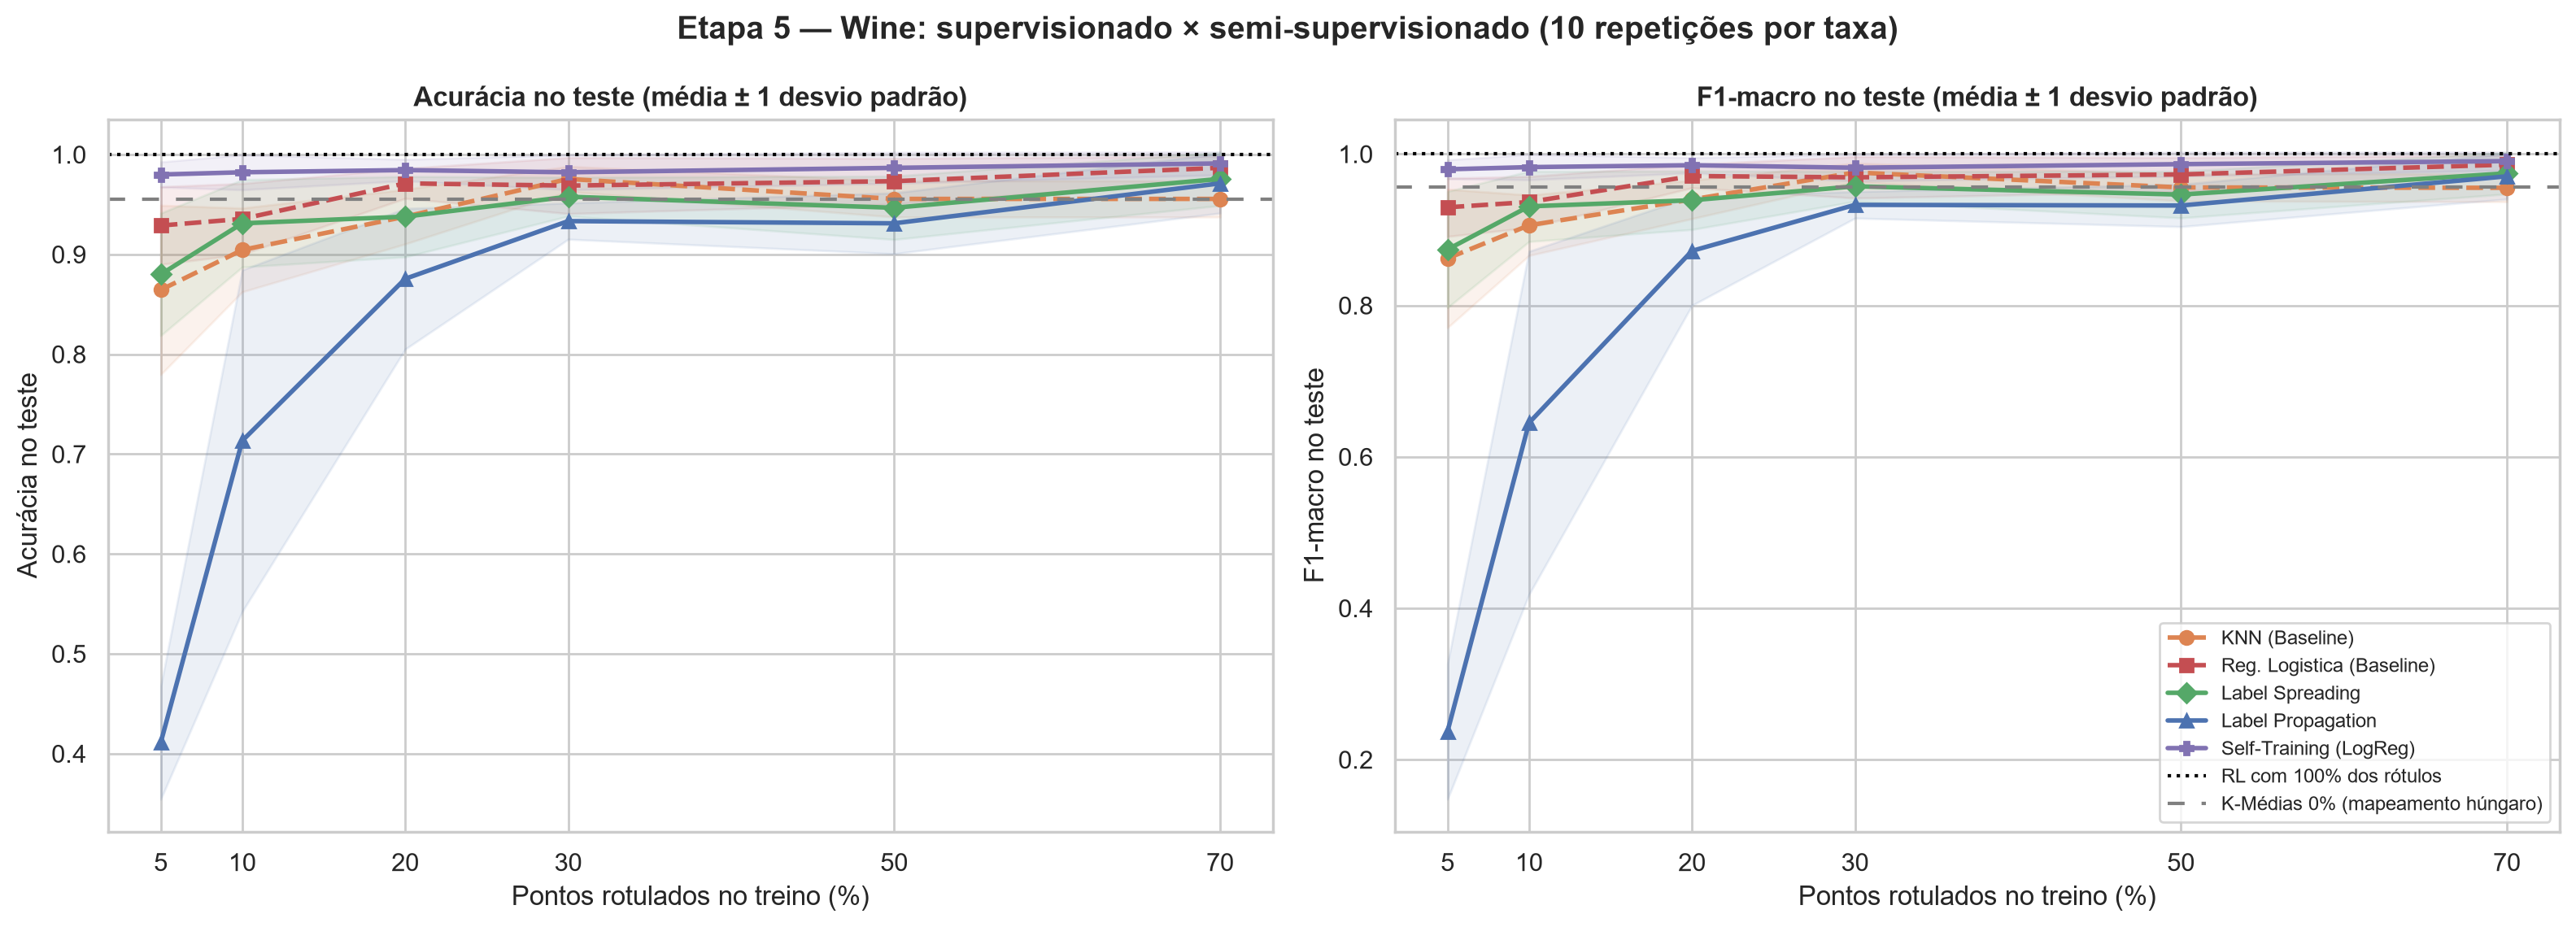
\includegraphics[width=\textwidth, keepaspectratio]{figuras/E5_wine_curva_aprendizado.png}
    \caption{Wine: acurácia e F1-macro no teste em função da taxa de rótulos (média $\pm$ 1 desvio padrão).}
    \label{fig:curva_wine}
\end{figure}

No Wine, o \textit{Self-Training} com Regressão Logística é o melhor método em todas as taxas. Com apenas 7 vinhos rotulados (5\%), atinge F1 = 0,980, contra 0,930 da Regressão Logística e 0,862 do KNN. A acurácia média do \textit{Self-Training} considerando todas as taxas foi de 98,44\%. O \textit{Label Propagation}, por outro lado, colapsa com poucos rótulos (F1 = 0,237 a 5\% e 0,645 a 10\%) e só se recupera a partir de 30\%. Com 70\% dos rótulos, o \textit{Self-Training} e a Regressão Logística convergem para cerca de 0,99.

\subsection{GANHO DO SEMI-SUPERVISIONADO E TESTE DE WILCOXON}

Para cada taxa, o melhor método semi-supervisionado de cada base (o \textit{Self-Training}, que teve o maior F1 médio considerando todas as taxas) foi comparado com cada \textit{baseline} pelo teste de Wilcoxon sobre as repetições pareadas (Figura \ref{fig:wilcoxon} e Tabela \ref{tab:wilcoxon}). É importante observar que, com as 5 repetições do Breast Cancer, o menor p-valor bicaudal possível é $2/2^5 = 0{,}0625$. Portanto, \textbf{nenhuma} diferença nessa base pode ser declarada significativa a 5\%. Com as 10 repetições do Wine, o mínimo é $2/2^{10} \approx 0{,}002$.

\begin{figure}[htbp]
    \centering
    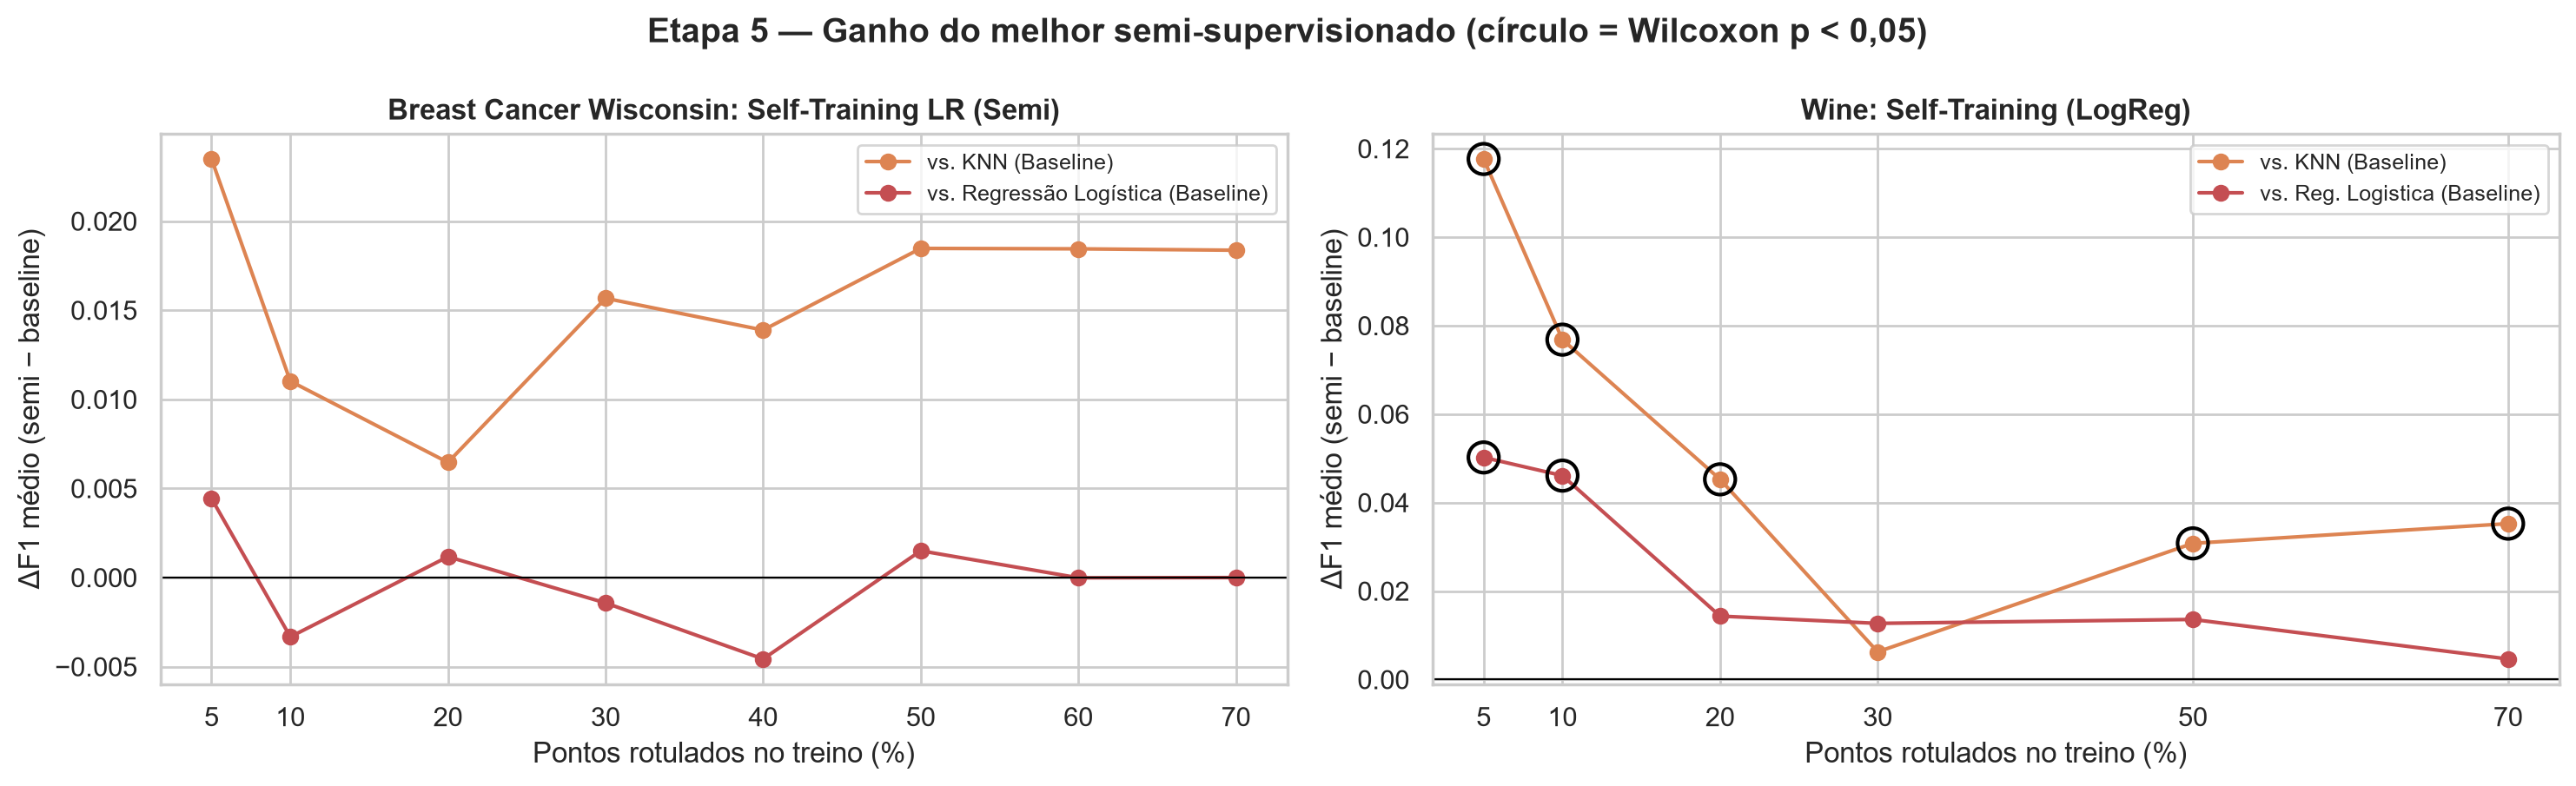
\includegraphics[width=\textwidth, keepaspectratio]{figuras/E5_wilcoxon_ganho.png}
    \caption{Ganho médio de F1-macro do \textit{Self-Training} sobre cada \textit{baseline}. Os círculos indicam diferenças significativas no teste de Wilcoxon ($p < 0{,}05$).}
    \label{fig:wilcoxon}
\end{figure}

\begin{table}[htbp]
\centering
\caption{\textit{Self-Training} LR contra a Regressão Logística nas taxas comuns às duas bases: ganho médio de F1-macro, número de repetições vencidas e p-valor do teste de Wilcoxon.}
\label{tab:wilcoxon}
\footnotesize
\begin{tabular}{ccccccc}
\toprule
 & \multicolumn{3}{c}{\textbf{Breast Cancer (5 repetições)}} & \multicolumn{3}{c}{\textbf{Wine (10 repetições)}} \\
\cmidrule(lr){2-4} \cmidrule(lr){5-7}
\textbf{Taxa} & $\Delta F1$ & \textbf{Vitórias} & \textbf{p} & $\Delta F1$ & \textbf{Vitórias} & \textbf{p} \\
\midrule
0,05 & $+$0,004 & 3/5 & 0,625 & $+$0,050 & 8/10 & \textbf{0,008} \\
0,10 & $-$0,003 & 1/5 & 0,500 & $+$0,046 & 9/10 & \textbf{0,004} \\
0,20 & $+$0,001 & 2/5 & 1,000 & $+$0,014 & 6/10 & 0,094 \\
0,30 & $-$0,001 & 1/5 & 1,000 & $+$0,013 & 5/10 & 0,063 \\
0,50 & $+$0,002 & 2/5 & 0,875 & $+$0,014 & 5/10 & 0,141 \\
0,70 & 0,000 & 0/5 & 1,000 & $+$0,005 & 3/10 & 0,625 \\
\bottomrule
\end{tabular}
\end{table}

No Wine, o \textit{Self-Training} supera a Regressão Logística de forma significativa com 5\% e 10\% de rótulos (ganhos de $+$0,050 e $+$0,046), e supera o KNN de forma significativa em quase todas as taxas. A partir de 20\%, a vantagem sobre a Regressão Logística deixa de ser significativa e diminui até $+$0,005 a 70\%. No Breast Cancer, os ganhos sobre a Regressão Logística oscilam em torno de zero em todas as taxas, e os ganhos sobre o KNN, embora consistentes (o \textit{Self-Training} vence as 5 repetições a partir de 30\%), não podem atingir significância com 5 repetições.

\subsection{MATRIZES DE CONFUSÃO}

As Figuras \ref{fig:matriz_bc} e \ref{fig:matriz_wine} mostram as matrizes de confusão do \textit{Self-Training} em execuções representativas, isto é, na repetição cujo F1 é o mais próximo da média da taxa, com 5\% e 70\% de rótulos.

\begin{figure}[htbp]
    \centering
    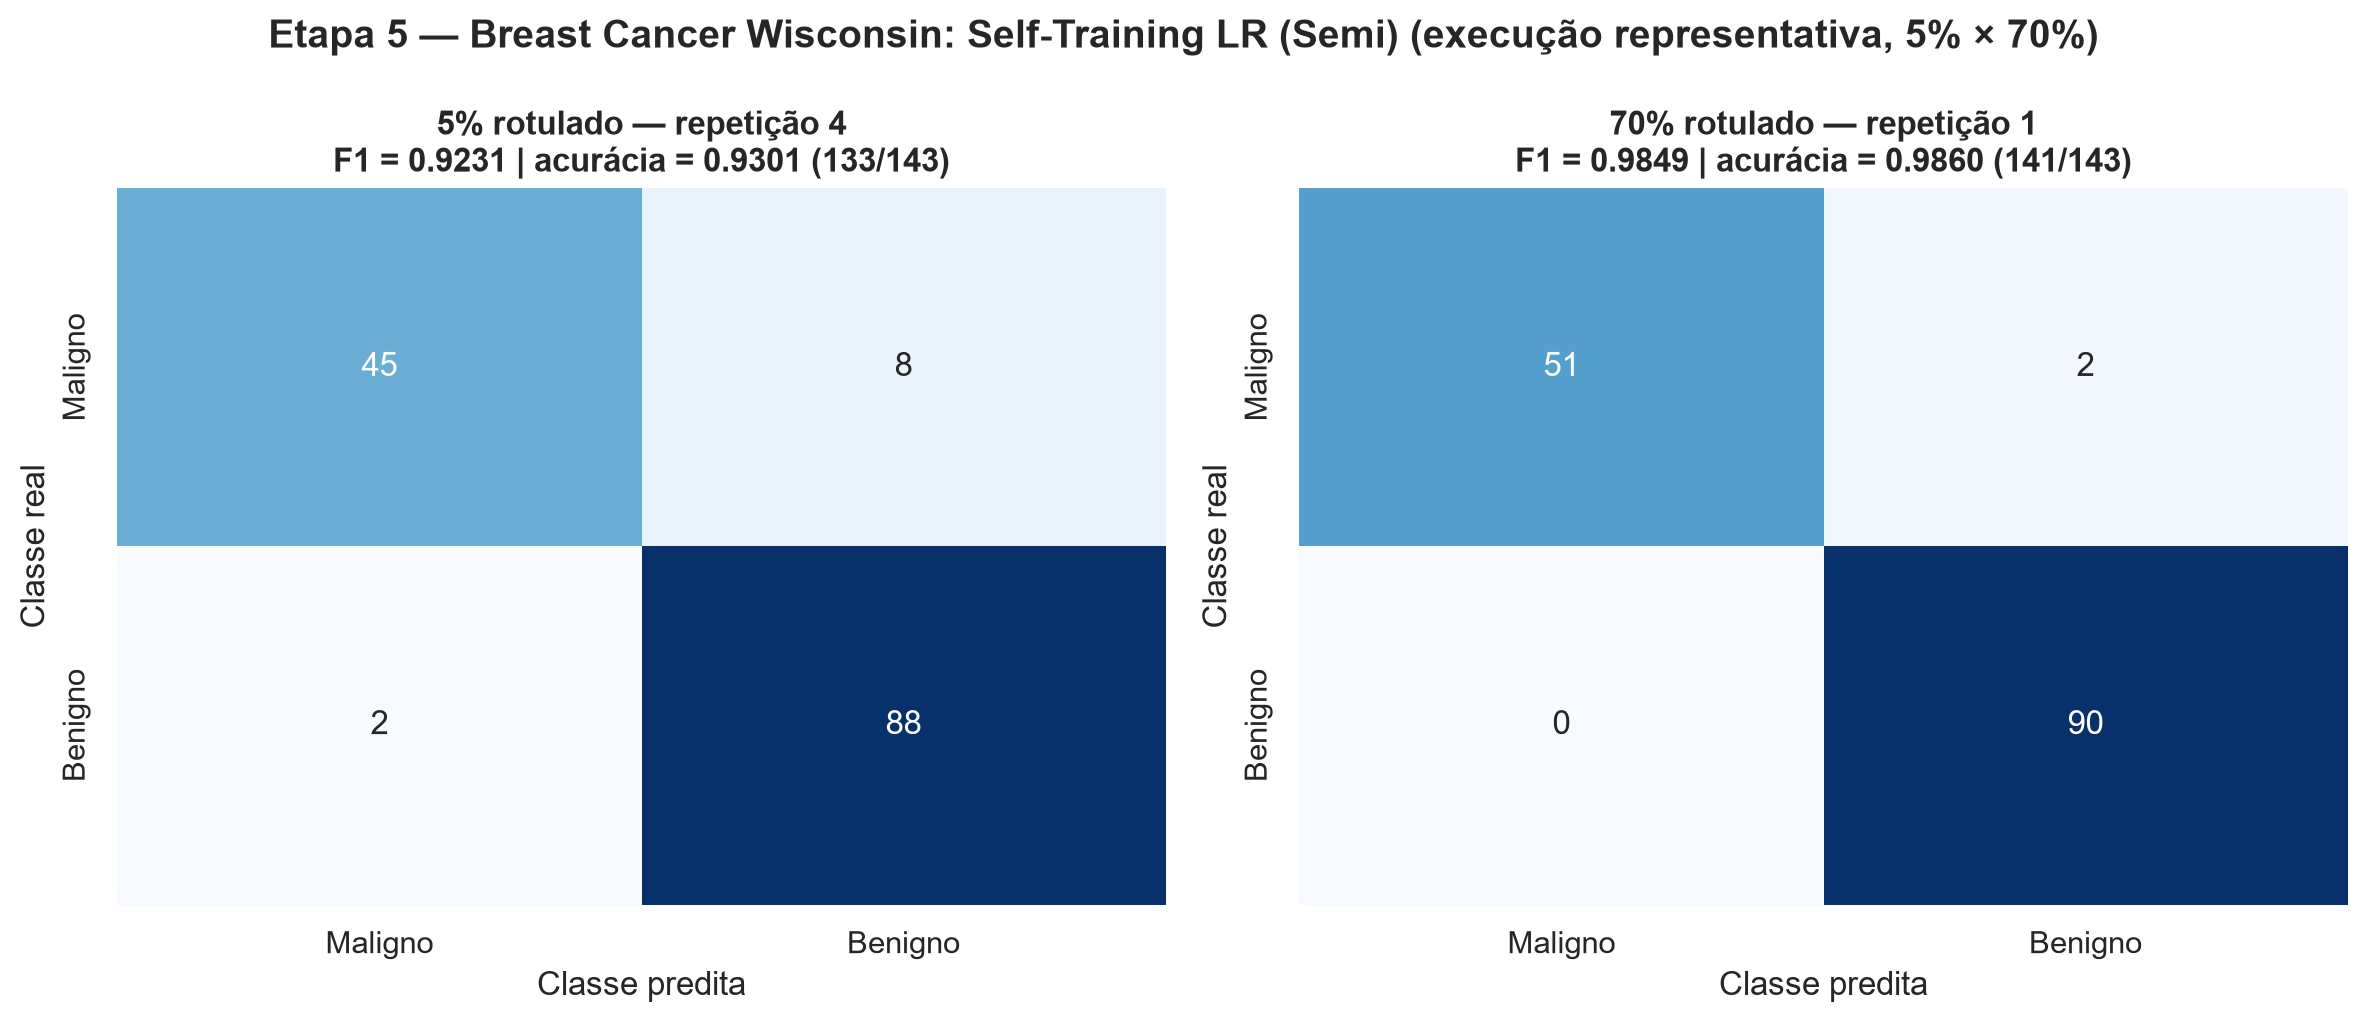
\includegraphics[width=0.9\textwidth, keepaspectratio]{figuras/E5_breast_cancer_matriz_representativa.png}
    \caption{Breast Cancer Wisconsin: matrizes de confusão do \textit{Self-Training} LR com 5\% e 70\% de rótulos (execuções representativas).}
    \label{fig:matriz_bc}
\end{figure}

No Breast Cancer, com 5\% de rótulos, o modelo acerta 133 dos 143 pacientes de teste (93,01\% de acurácia), com 8 falsos negativos e 2 falsos positivos. Com 70\% de rótulos, acerta 141 de 143 (98,60\%), com apenas 2 falsos negativos e nenhum falso positivo. O ganho de 5,59 pontos percentuais corrige 8 diagnósticos incorretos e, principalmente, reduz os falsos negativos, que são o erro mais grave em um contexto de triagem.

\begin{figure}[htbp]
    \centering
    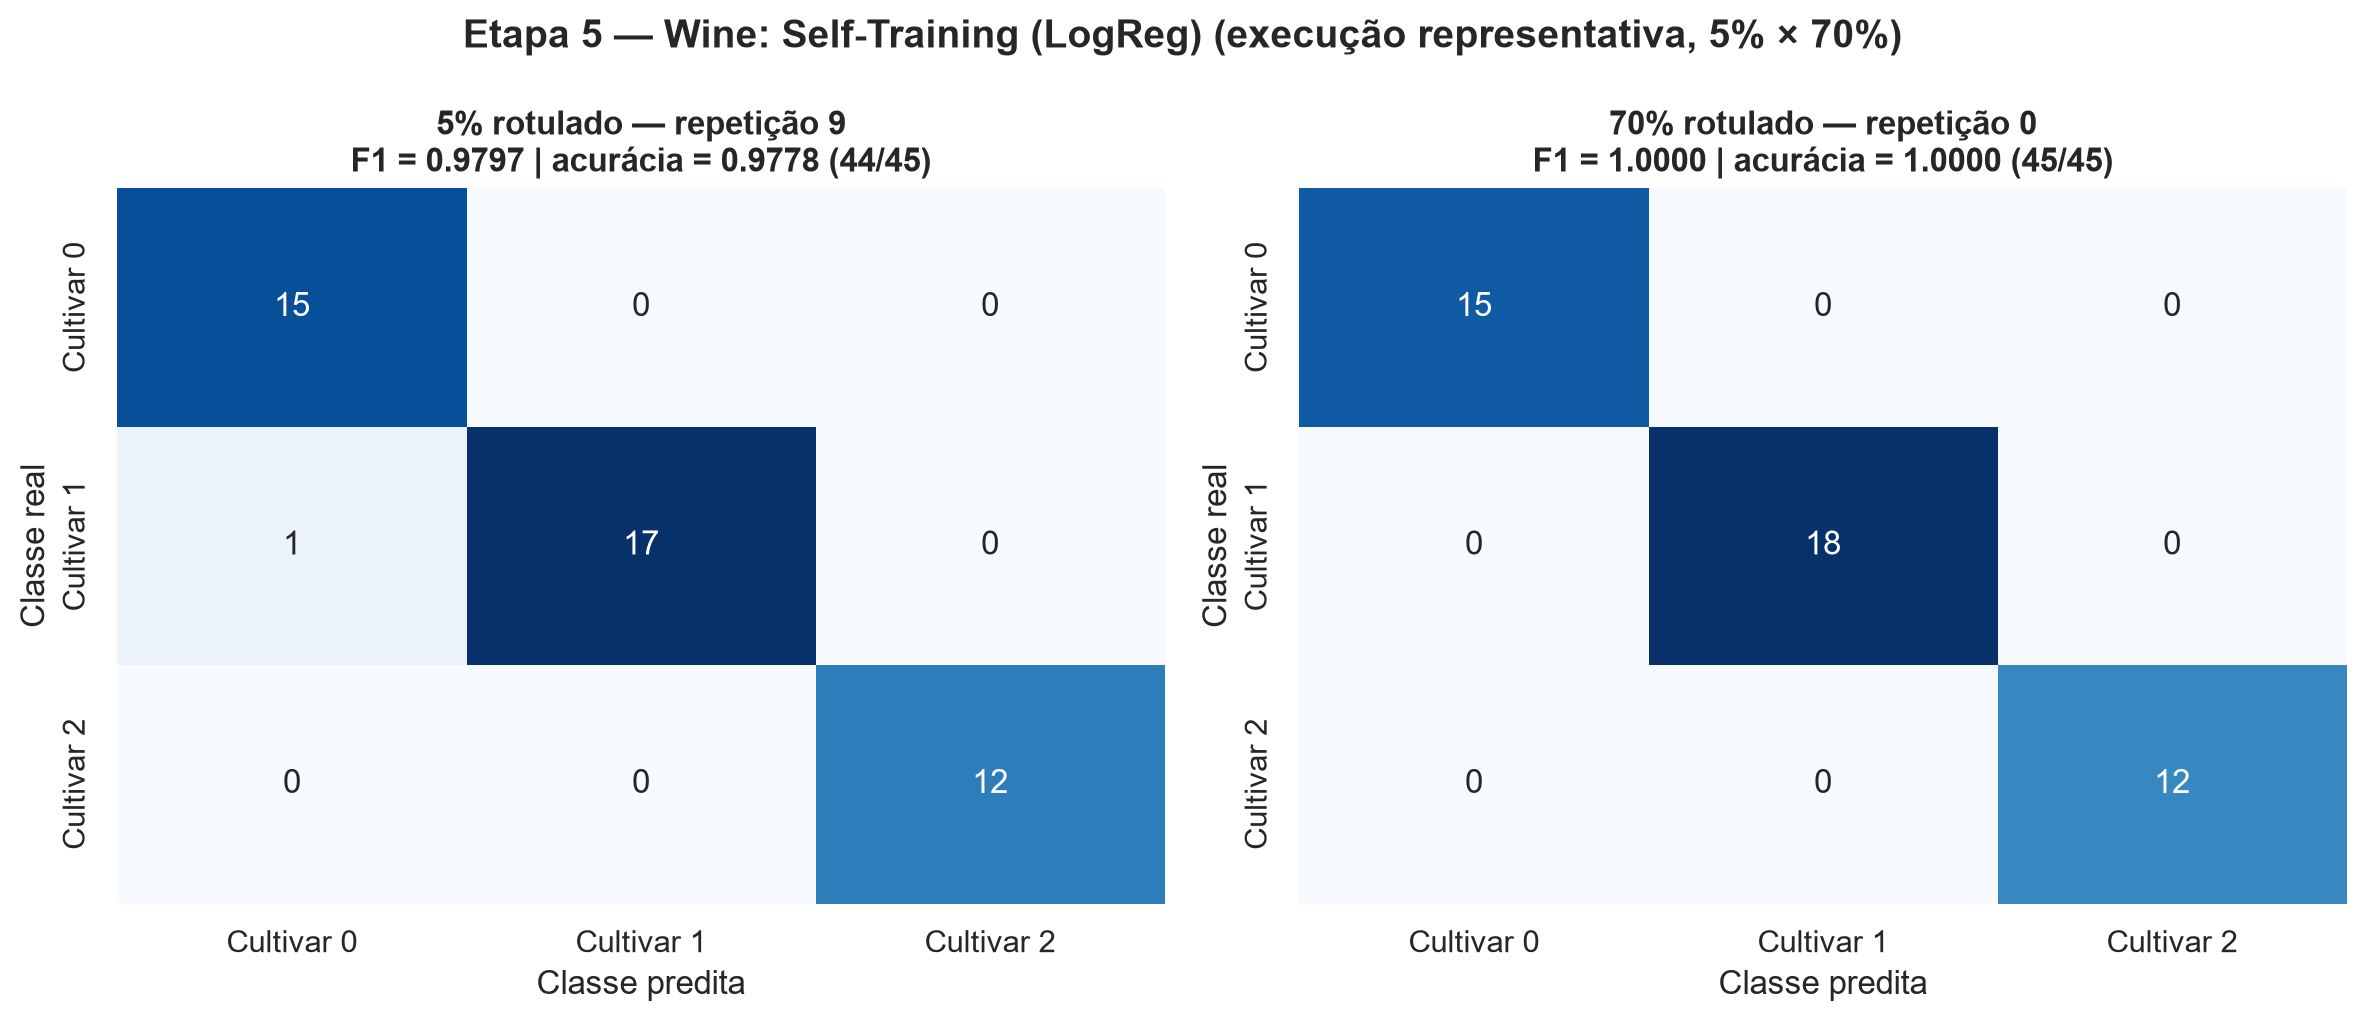
\includegraphics[width=0.9\textwidth, keepaspectratio]{figuras/E5_wine_matriz_representativa.png}
    \caption{Wine: matrizes de confusão do \textit{Self-Training} LR com 5\% e 70\% de rótulos (execuções representativas).}
    \label{fig:matriz_wine}
\end{figure}

No Wine, com 5\% de rótulos, o modelo acerta 44 dos 45 vinhos de teste (97,78\%), com um único erro (um vinho da cultivar 1 classificado como cultivar 0). Com 70\% de rótulos, acerta todos os 45 (100\%). Como o conjunto de teste tem apenas 45 amostras, cada erro corresponde a 2,22 pontos percentuais de acurácia.

\subsection{PROPAGAÇÃO DE RÓTULOS E SENSIBILIDADE AOS HIPERPARÂMETROS}

A Figura \ref{fig:propagacao_wine} ilustra o funcionamento do \textit{Label Spreading} no Wine com 5\% de rótulos: a partir de apenas 7 pontos rotulados, os rótulos são propagados pelo grafo de similaridade para todo o treino, com 86,5\% de acerto nos pontos não rotulados (avaliação transdutiva). Os erros se concentram nas regiões de transição em que a cultivar 1 encosta nas cultivares 0 e 2, e coincidem com os pontos de menor confiança da inferência.

\begin{figure}[htbp]
    \centering
    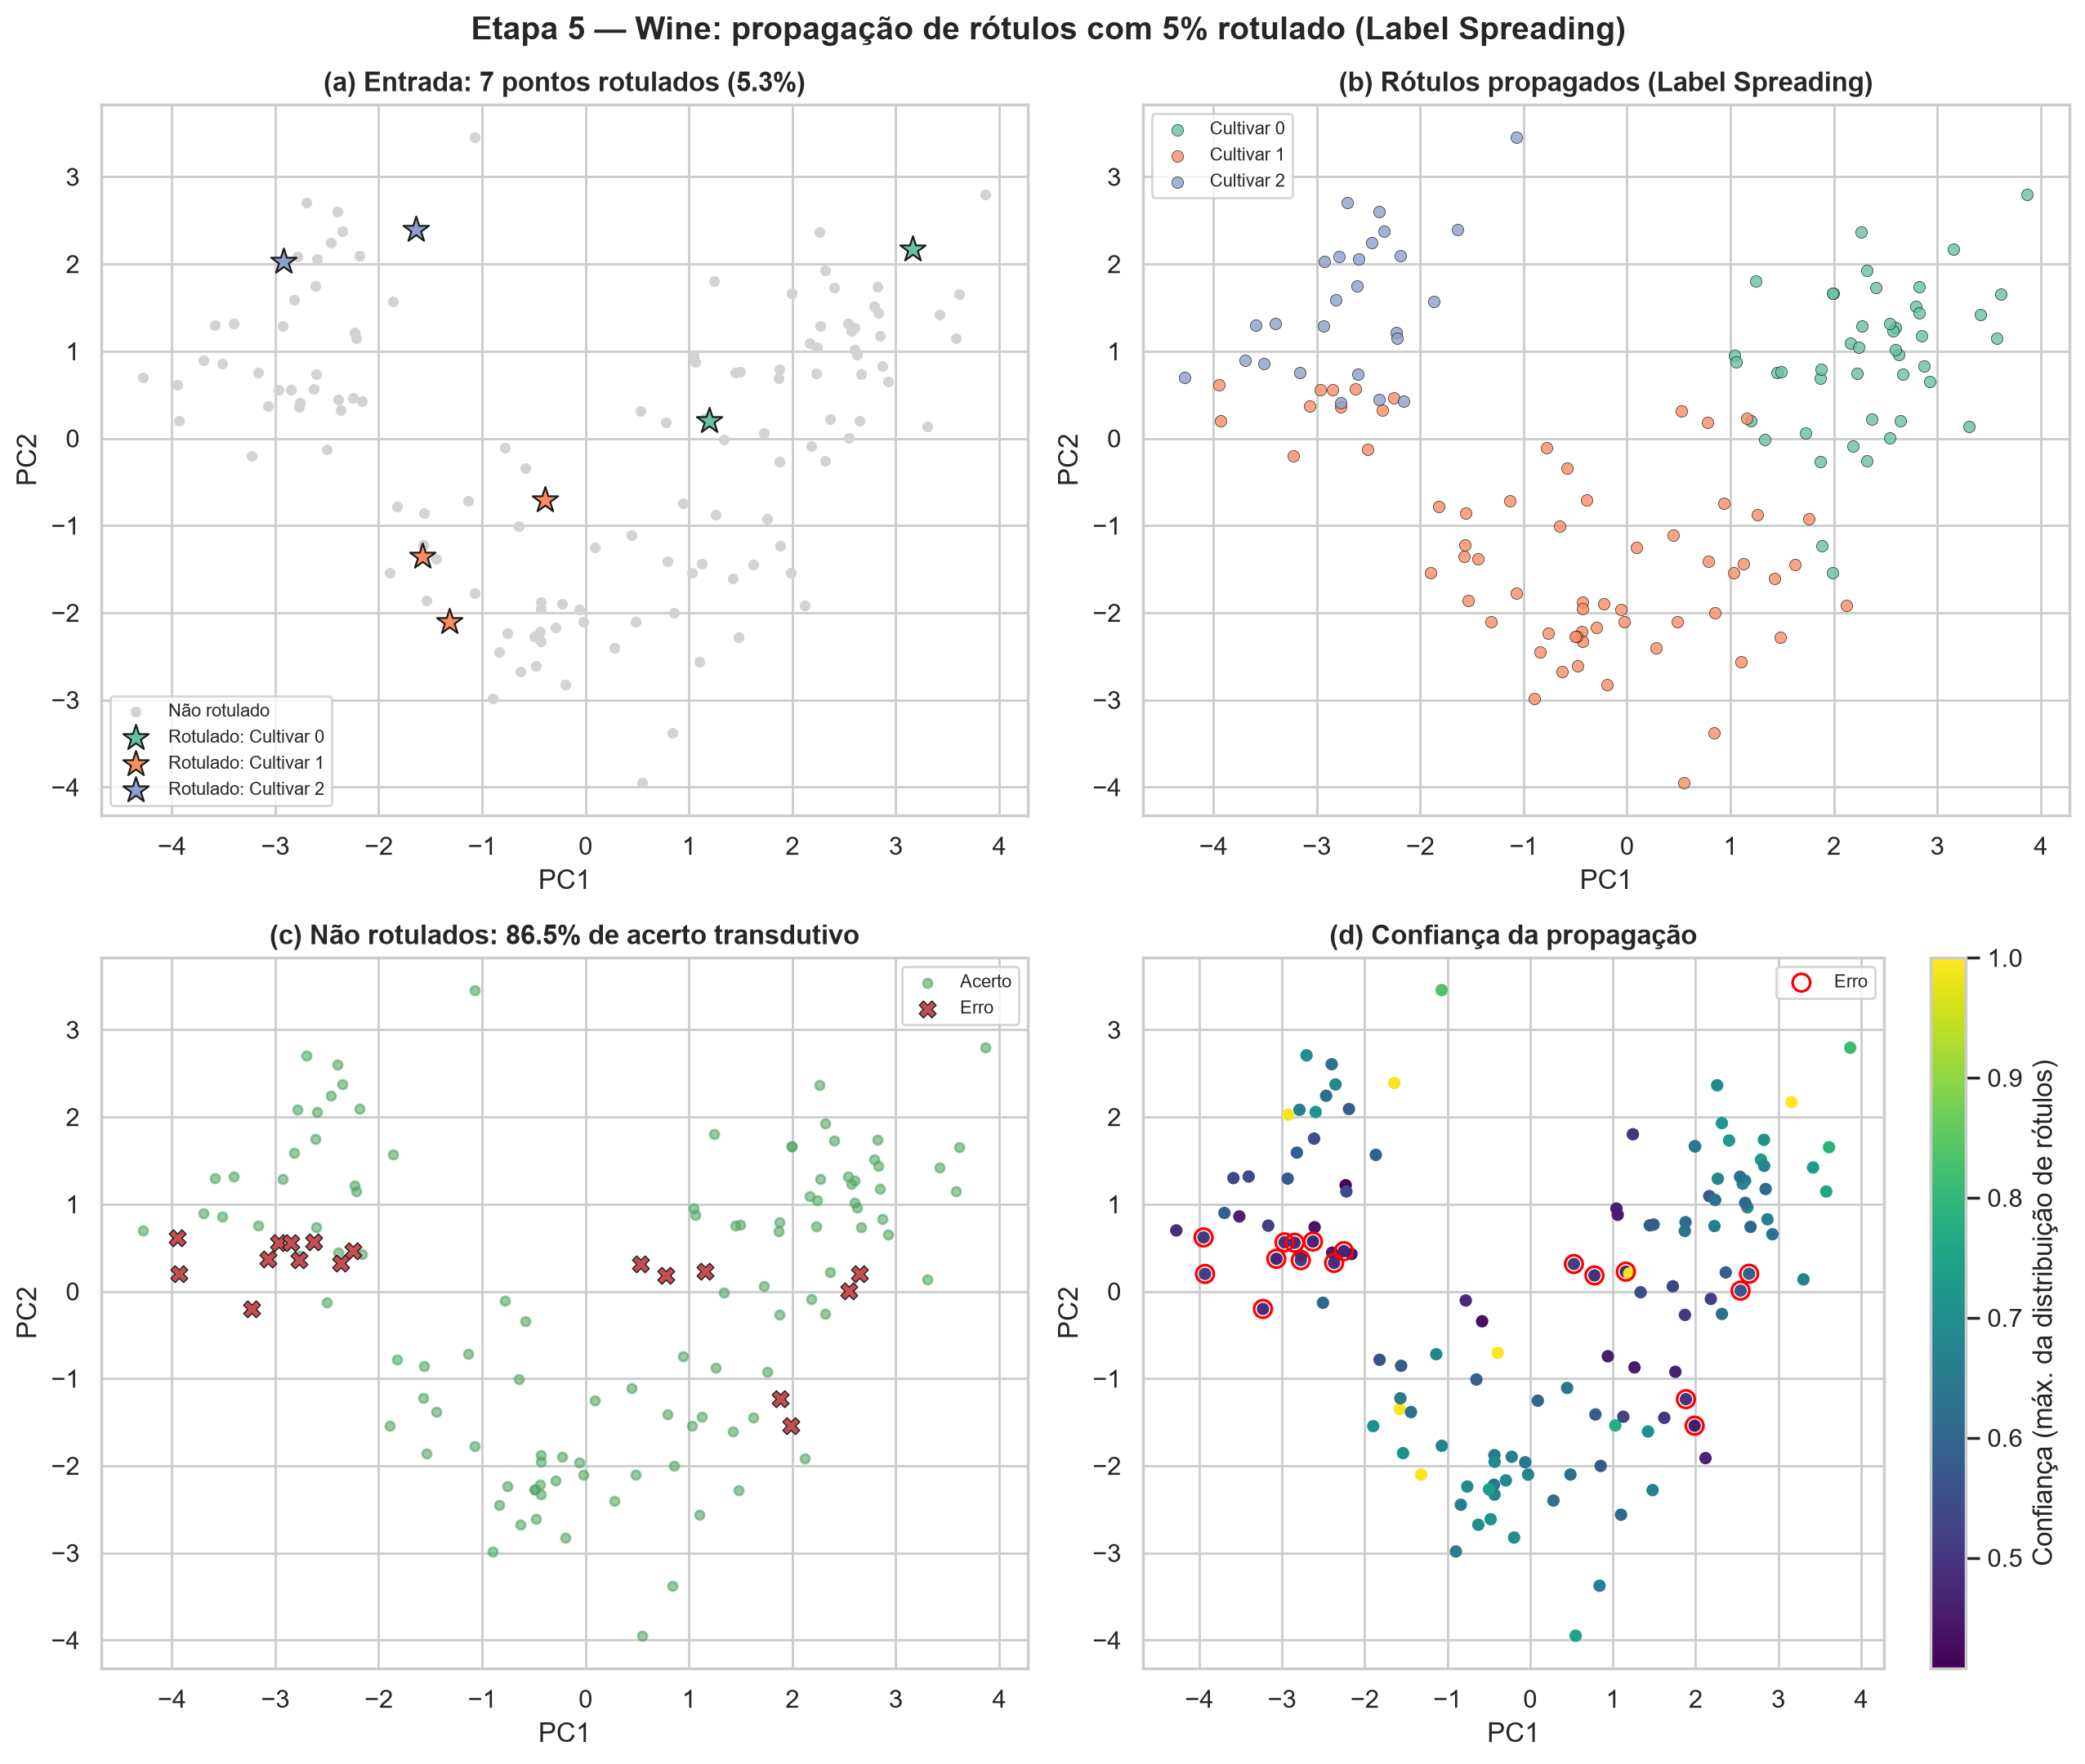
\includegraphics[width=0.85\textwidth, keepaspectratio]{figuras/E5_wine_propagacao_rotulos.png}
    \caption{Wine: \textit{Label Spreading} com 5\% de rótulos no espaço PCA 2D: (a) pontos rotulados, (b) rótulos inferidos, (c) acertos e erros nos não rotulados e (d) confiança da inferência.}
    \label{fig:propagacao_wine}
\end{figure}

Os métodos foram também avaliados variando um hiperparâmetro por vez a partir da configuração dos \textit{scripts}. Os principais achados foram:

\begin{itemize}
    \item \textbf{\textit{Self-Training}} (Figura \ref{fig:sens_self_training}): no Wine com 5\% de rótulos, o limiar de 0,80 faz com que 93,6\% dos pontos não rotulados recebam pseudo-rótulo, com 97,6\% de acerto, levando a F1 = 0,980. Com o limiar de 0,95, apenas 45,2\% são pseudo-rotulados e o F1 cai para 0,855. Com limiares muito altos, quase nada é pseudo-rotulado e o método se reduz à própria Regressão Logística.
    \item \textbf{\textit{Label Spreading} no Wine}: o colapso observado no \textit{Label Propagation} também ocorre no \textit{Label Spreading} quando o núcleo fica largo demais ($\gamma = 0{,}25/13$, F1 = 0,19) ou a suavização forte demais ($\alpha = 0{,}95$, F1 = 0,25). Com $\gamma = 2/13$, por outro lado, o F1 a 5\% chegaria a 0,922.
    \item \textbf{\textit{Label Spreading} no Breast Cancer}: com \texttt{n\_neighbors} = 3, o grafo kNN se fragmenta e 26,6\% dos pontos de teste ficam sem nenhum rótulo alcançável a 5\% (o \texttt{scikit-learn} atribui a eles a classe de índice 0), o que derruba o F1 para 0,758.
    \item \textbf{KNN (\textit{baseline})}: no Wine a 5\%, o \textit{script} usa $k = \min(5, 7/2) = 3$ (F1 = 0,862). Com $k = 5$ e apenas 7 rótulos, o F1 cairia para 0,330, e com $k = 1$ subiria para 0,873. Como as hipóteses comparam sempre com o \textbf{melhor} \textit{baseline} de cada taxa (a Regressão Logística, nesse caso), a escolha de $k$ não infla os ganhos reportados.
\end{itemize}

\begin{figure}[htbp]
    \centering
    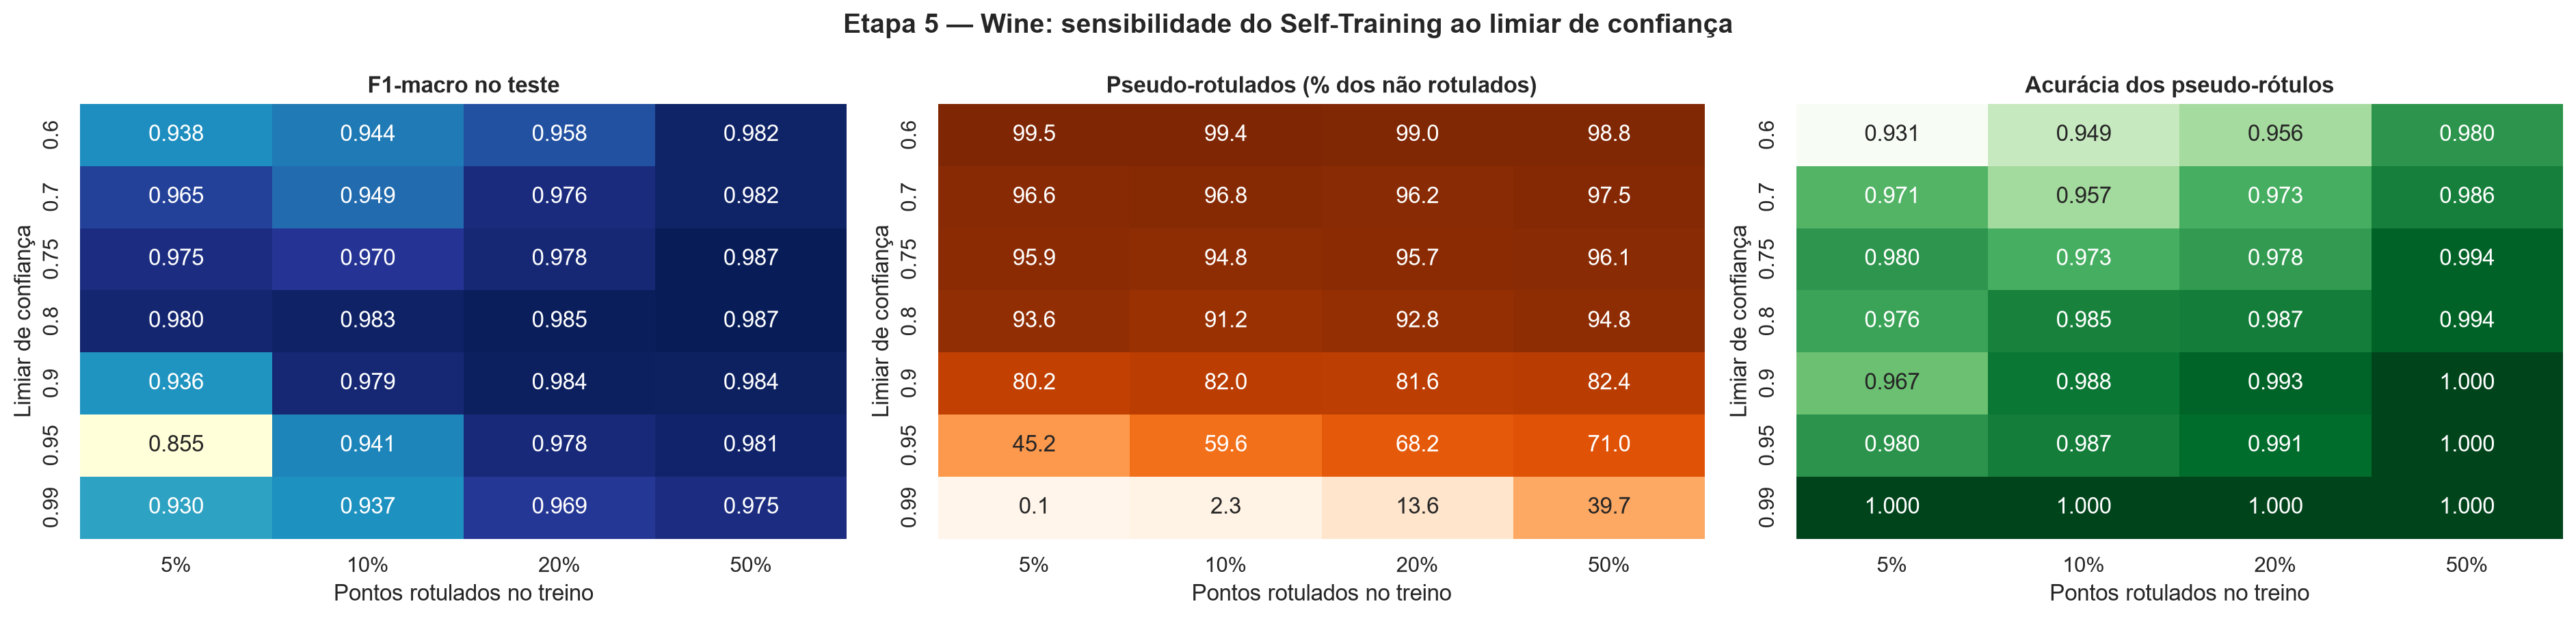
\includegraphics[width=\textwidth, keepaspectratio]{figuras/E5_wine_sensibilidade_self_training.png}
    \caption{Wine: sensibilidade do \textit{Self-Training} ao limiar de confiança: F1-macro no teste, fração de pontos pseudo-rotulados e acurácia dos pseudo-rótulos.}
    \label{fig:sens_self_training}
\end{figure}

Em termos de custo computacional, todos os modelos treinam em milissegundos nessas bases. O \textit{Self-Training} é o mais caro (da ordem de 20 ms, pois retreina a Regressão Logística a cada iteração), e o KNN, o mais barato (menos de 1 ms).

\chapter[Avaliação e Interpretação]{AVALIAÇÃO E INTERPRETAÇÃO}

Este capítulo corresponde à Etapa 6 do processo KDD, na qual o conhecimento sobre os dados e sobre os modelos é sintetizado. Como lembra a proposta do trabalho, os dados são compreendidos por meio dos modelos.

\section{ESPECTRO COMPLETO DE SUPERVISÃO}

A Figura \ref{fig:espectro} e a Tabela \ref{tab:espectro} reúnem, em uma mesma escala, o desempenho obtido com 0\% de rótulos (K-Médias com mapeamento húngaro), com taxas intermediárias (melhor \textit{baseline} e melhor semi-supervisionado de cada taxa) e com 100\% de rótulos (classificadores supervisionados treinados com todo o treino).

\begin{figure}[htbp]
    \centering
    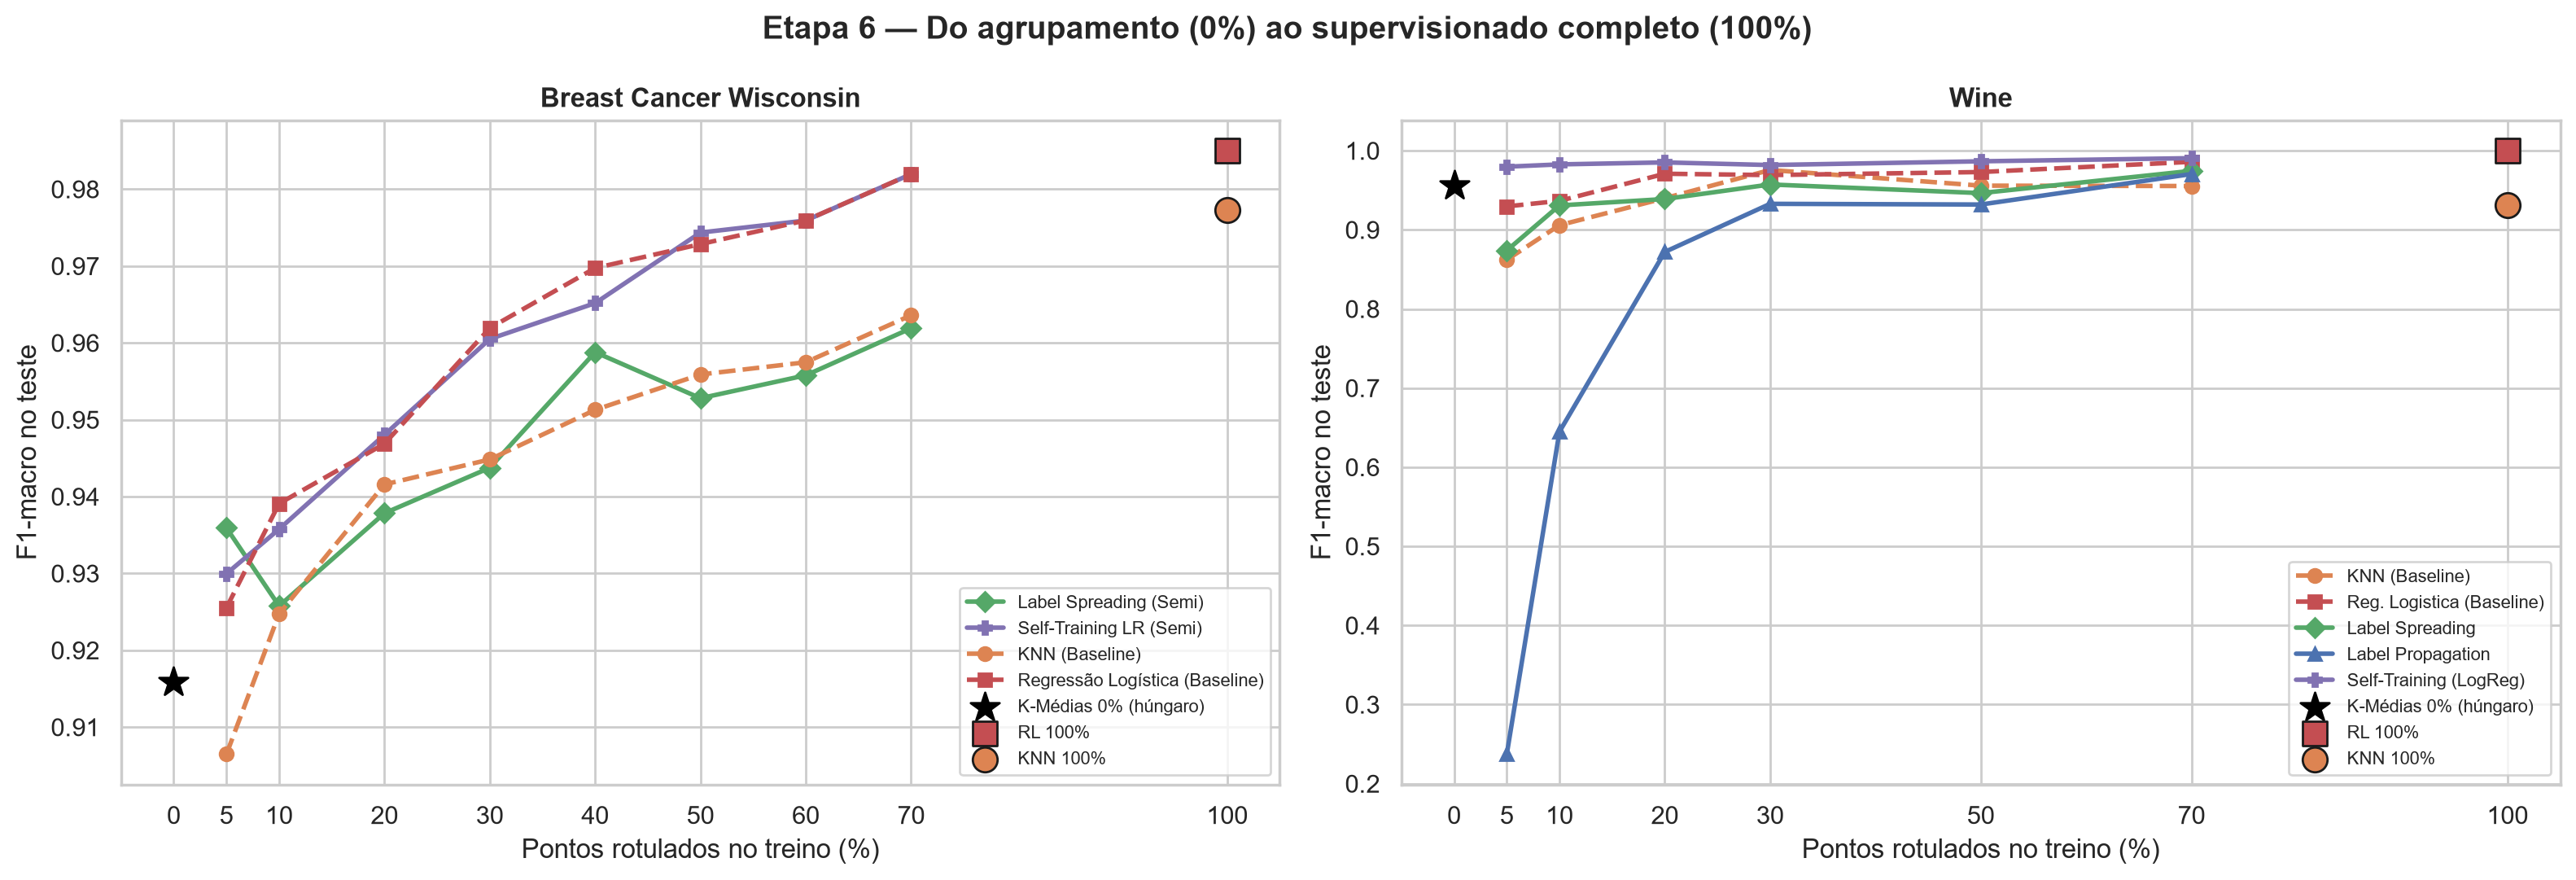
\includegraphics[width=\textwidth, keepaspectratio]{figuras/E6_espectro_supervisao.png}
    \caption{F1-macro no teste ao longo de todo o espectro de supervisão, do agrupamento (0\%) ao supervisionado completo (100\%).}
    \label{fig:espectro}
\end{figure}

\begin{table}[htbp]
\centering
\caption{F1-macro no teste ao longo do espectro de supervisão.}
\label{tab:espectro}
\footnotesize
\begin{tabular}{lccccccc}
\toprule
 & \textbf{0\%} & \multicolumn{2}{c}{\textbf{5\%}} & \multicolumn{2}{c}{\textbf{70\%}} & \multicolumn{2}{c}{\textbf{100\%}} \\
\cmidrule(lr){3-4} \cmidrule(lr){5-6} \cmidrule(lr){7-8}
\textbf{Base} & \textbf{K-Médias} & \textbf{Baseline} & \textbf{Semi} & \textbf{Baseline} & \textbf{Semi} & \textbf{RL} & \textbf{KNN} \\
\midrule
Breast Cancer & 0,916 & 0,926 & 0,936 & 0,982 & 0,982 & 0,985 & 0,977 \\
Wine & 0,956 & 0,930 & 0,980 & 0,986 & 0,991 & 1,000 & 0,931 \\
\bottomrule
\end{tabular}
\end{table}

Dois aspectos se destacam. Primeiro, no Wine, o K-Médias sem nenhum rótulo (0,956) supera a Regressão Logística treinada com 5\% dos rótulos (0,930), e o \textit{Self-Training} com 5\% (0,980) já se aproxima do desempenho supervisionado completo. Segundo, no Breast Cancer, o ganho entre 0\% e 100\% é obtido de forma gradual, e o melhor método em cada taxa alterna entre semi-supervisionados e a Regressão Logística.

\section{O QUE OS MODELOS REVELAM SOBRE OS ATRIBUTOS}

Treinada com 100\% dos rótulos no espaço padronizado, a Regressão Logística tem coeficientes comparáveis entre si: o sinal indica a direção do efeito, e a magnitude, a importância \textit{condicional} (dados os demais atributos).

No \textbf{Breast Cancer}, os atributos com maiores coeficientes (\texttt{worst texture}, \texttt{radius error}, \texttt{worst symmetry}, \texttt{worst concave points} e \texttt{area error}) diferem do ranking univariado da ANOVA (correlação de Spearman de 0,589 entre os rankings). Isso é consequência da forte multicolinearidade observada na Etapa 3: a Regressão Logística distribui o peso entre as variáveis redundantes de tamanho, de modo que a importância condicional difere da marginal. Os \textbf{pontos côncavos} aparecem nos dois rankings e são o marcador mais robusto de malignidade.

No \textbf{Wine}, há maior concordância entre os rankings (Spearman de 0,670): \texttt{proline}, \texttt{flavanoids}, \texttt{alcohol} e \texttt{color\_intensity} estão entre os cinco primeiros nos dois casos.

\section{ANÁLISE DE ERROS}

Para cada amostra de teste, foi calculada a taxa de erro considerando todos os modelos, taxas e repetições do experimento semi-supervisionado. A Figura \ref{fig:erros_bc} mostra o resultado para o Breast Cancer.

\begin{figure}[htbp]
    \centering
    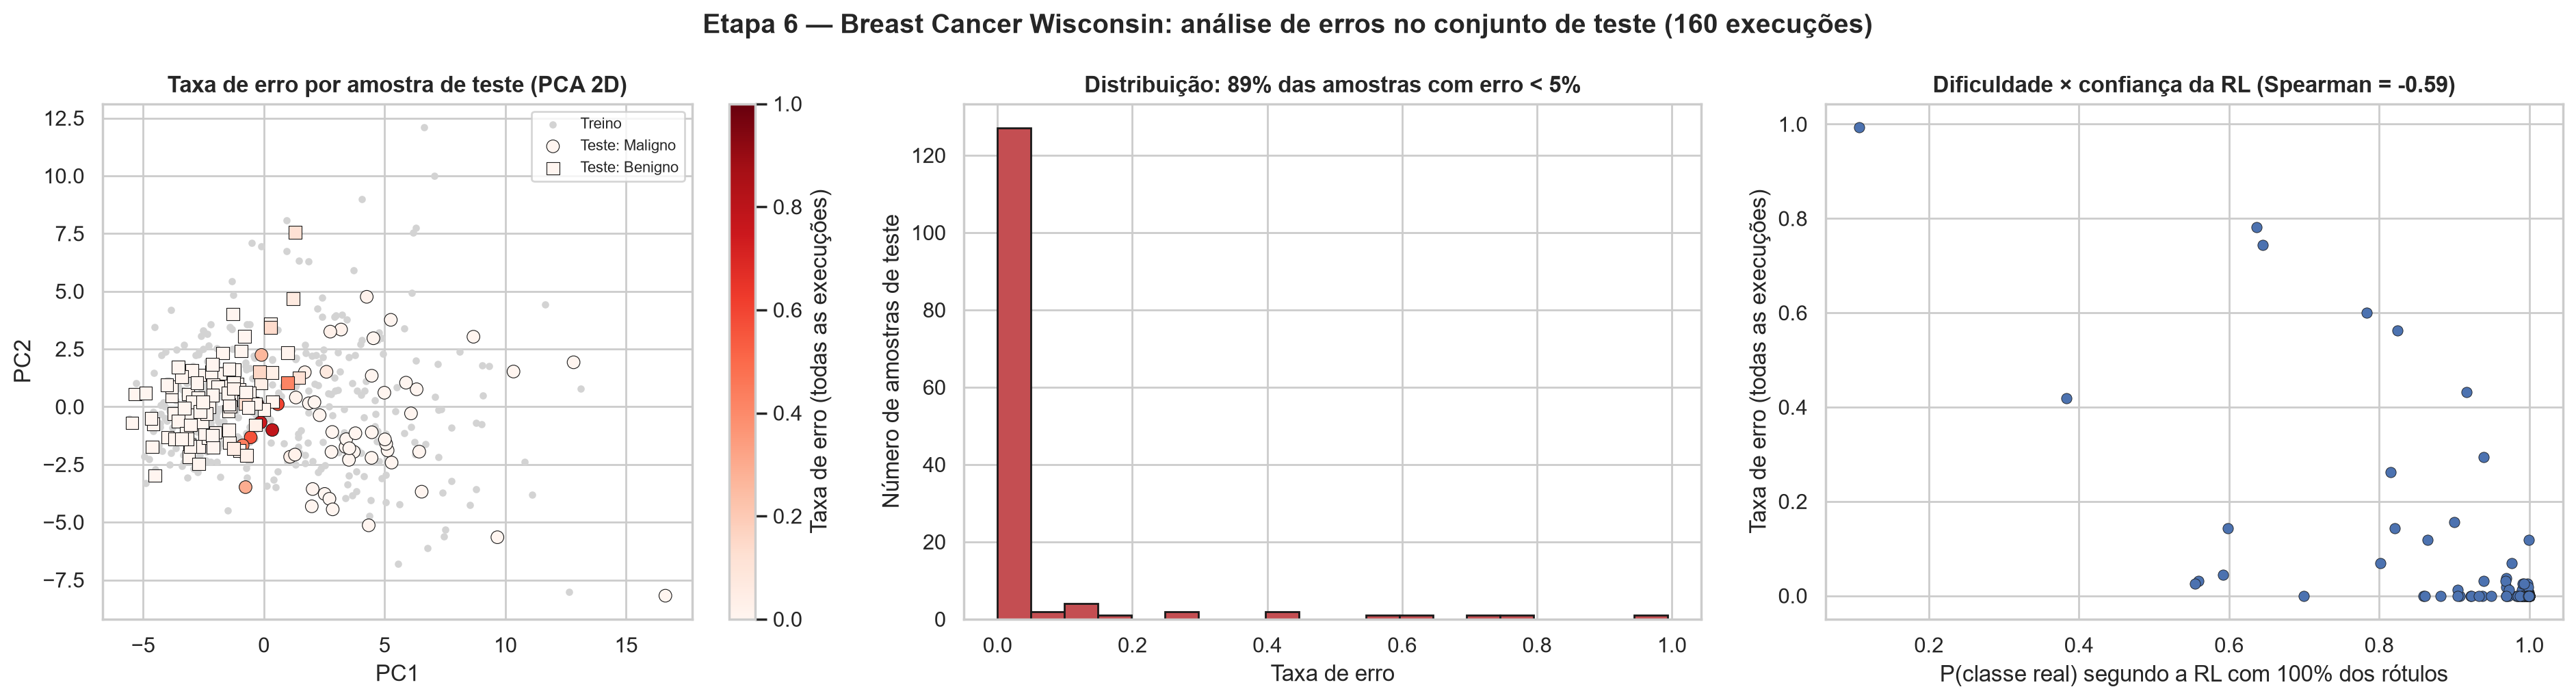
\includegraphics[width=\textwidth, keepaspectratio]{figuras/E6_breast_cancer_analise_erros.png}
    \caption{Breast Cancer Wisconsin: taxa de erro por amostra de teste, considerando as 160 execuções do experimento, e sua relação com a probabilidade atribuída à classe real pela Regressão Logística com 100\% dos rótulos.}
    \label{fig:erros_bc}
\end{figure}

No Breast Cancer, 88,8\% das amostras de teste quase nunca são classificadas incorretamente (taxa de erro menor que 5\%). As seis amostras mais difíceis são todas \textbf{malignas classificadas como benignas}, ou seja, falsos negativos, o erro mais grave em um contexto de triagem. Elas ficam na fronteira entre as classes no PCA. Uma delas é classificada incorretamente em 99,4\% das execuções, e até a Regressão Logística com 100\% dos rótulos lhe atribui probabilidade de malignidade de apenas 0,107. Trata-se de um caso atípico, possivelmente com rótulo ruidoso, o que não é possível verificar com os dados disponíveis. No Wine, a proporção de amostras ``fáceis'' é menor (57,8\%), porque o colapso do \textit{Label Propagation} com poucos rótulos produz muitos erros em várias execuções.

\section{REVISÃO DAS HIPÓTESES}

Como o processo KDD não é linear, a mineração pode contradizer as hipóteses iniciais. A Tabela \ref{tab:veredito} aplica os critérios objetivos definidos na Etapa 1.

\begin{table}[htbp]
\centering
\caption{Revisão das hipóteses formuladas na Etapa 1.}
\label{tab:veredito}
\footnotesize
\begin{tabular}{p{0.6cm} p{2.4cm} p{8.4cm} p{2.6cm}}
\toprule
\textbf{\#} & \textbf{Base} & \textbf{Evidência} & \textbf{Resultado} \\
\midrule
H1 & Breast Cancer & F1 da Regressão Logística com 100\% dos rótulos = 0,985 & Confirmada \\
\addlinespace
H2 & Breast Cancer & 5\%: \textit{Label Spreading} $-$ RL = $+$0,010 (vence 4/5; $p = 0{,}125$). 10\%: \textit{Self-Training} $-$ RL = $-$0,003 (vence 1/5; $p = 0{,}500$) & 5\%: inconclusiva; 10\%: refutada \\
\addlinespace
H2 & Wine & 5\%: \textit{Self-Training} $-$ RL = $+$0,050 (vence 8/10; $p = 0{,}008$). 10\%: $+$0,046 (vence 9/10; $p = 0{,}004$) & Confirmada \\
\addlinespace
H3 & Breast Cancer & $\Delta F1$ (melhor semi $-$ melhor \textit{baseline}): 5\% = $+$0,010; 70\% = 0,000 & Confirmada \\
\addlinespace
H3 & Wine & $\Delta F1$: 5\% = $+$0,050; 70\% = $+$0,005 & Confirmada \\
\addlinespace
H4 & Ambas & ARI do K-Médias: Wine = 0,908; Breast Cancer = 0,672 & Confirmada \\
\addlinespace
H5 & Breast Cancer & ARI: DBSCAN = 0,025; K-Médias = 0,672 & Confirmada \\
\addlinespace
H5 & Wine & ARI: DBSCAN = 0,602; K-Médias = 0,908 & Confirmada \\
\addlinespace
H6 & Breast Cancer & F1 do KNN: completo = 0,962; PCA 2D = 0,932 (96,9\%) & Confirmada \\
\addlinespace
H6 & Wine & F1 do KNN: completo = 0,963; PCA 2D = 0,978 (101,6\%) & Confirmada \\
\bottomrule
\end{tabular}
\end{table}

\section{SÍNTESE}

\textbf{O benefício do semi-supervisionado depende da estrutura dos dados, e não só da escassez de rótulos.} No Wine, as cultivares formam grupos compactos (ARI do K-Médias de 0,908), a hipótese de \textit{cluster} vale e os pontos não rotulados ajudam muito: com 5\% de rótulos, o \textit{Self-Training} supera a Regressão Logística em 0,050 de F1, com significância estatística. No Breast Cancer, a fronteira entre as classes é essencialmente linear (H1), e um modelo supervisionado simples com o viés indutivo adequado é tão bom quanto as alternativas semi-supervisionadas. A vantagem observada a 5\% diminui com mais rótulos (H3), mas não é estatisticamente sustentada.

\textbf{O agrupamento funciona como diagnóstico.} O caso com 0\% de rótulos antecipou onde o semi-supervisionado ajudaria: quando o K-Médias já recupera as classes (Wine), os dados não rotulados agregam informação; quando não recupera (Breast Cancer), não agregam.

\textbf{Sobre os modelos.} O \textit{Self-Training} com Regressão Logística foi o melhor semi-supervisionado em média nas duas bases, porque herda o viés linear da Regressão Logística e acrescenta pseudo-rótulos de boa qualidade, desde que o limiar de confiança seja adequado. Os métodos de grafo (\textit{Label Propagation} e \textit{Label Spreading}) mostraram-se muito sensíveis aos hiperparâmetros $\gamma$, $\alpha$ e \texttt{n\_neighbors}, que foram fixados \textit{a priori}. Ajustá-los exigiria dados rotulados de validação, justamente o recurso escasso nesse cenário. As diferenças entre a avaliação indutiva (teste) e a transdutiva (pontos não rotulados do treino) foram pequenas, no máximo cerca de 0,05 em F1, e não indicaram sobreajuste sistemático aos pontos não rotulados.

\textbf{Revisão do processo.} O resultado inconclusivo no Breast Cancer leva de volta à Etapa 1: a hipótese de que o semi-supervisionado ajuda quando há poucos rótulos precisa ser condicionada à estrutura de agrupamento dos dados e testada com repetições suficientes. Uma nova iteração do processo poderia (a) aumentar o número de repetições no Breast Cancer, (b) ajustar $\gamma$ e $\alpha$ dos métodos de grafo por validação cruzada sobre os poucos rótulos disponíveis e (c) ajustar o limiar de decisão para reduzir os falsos negativos.

\textbf{Limitações.} Foi usada uma única partição treino/teste. No Wine, o teste tem 45 amostras, de modo que um erro equivale a 2,2 pontos de acurácia. Os p-valores do teste de Wilcoxon são indicativos, pois todas as repetições usam o mesmo conjunto de teste. Por fim, os protocolos das duas bases diferem entre si (taxas, repetições, modelos e hiperparâmetros), e por isso as comparações entre as bases são qualitativas.

\section{PÓS-PROCESSAMENTO}

A Etapa 7, opcional, consistiu na exportação de todas as figuras e tabelas de métricas para uso neste relatório e na apresentação, e na formulação das seguintes recomendações práticas:

\begin{itemize}
    \item \textbf{Breast Cancer:} em um cenário com poucos laudos, uma Regressão Logística sobre atributos padronizados, treinada apenas com os casos rotulados, é a opção mais simples e mais fácil de auditar, e as alternativas semi-supervisionadas não mostraram vantagem estatisticamente sustentada sobre ela. Como os erros residuais são falsos negativos, o limiar de decisão deve ser escolhido priorizando a sensibilidade para a classe maligna. O modelo é um apoio à triagem e não substitui o diagnóstico do patologista.
    \item \textbf{Wine:} com apenas 7 vinhos rotulados, o \textit{Self-Training} com Regressão Logística já atinge F1 de 0,98 usando os demais vinhos sem rótulo, o que reduz o custo de rotulagem por análise especializada. O limiar de confiança deve ser escolhido com cuidado, pois limiares altos anulam o ganho.
    \item \textbf{Reprodutibilidade:} sementes fixas, versões das bibliotecas registradas e todas as métricas exportadas em arquivos CSV.
\end{itemize}

\chapter[Considerações Finais]{CONSIDERAÇÕES FINAIS}

Este trabalho aplicou as sete etapas do processo KDD a duas bases com atributos contínuos e rótulos discretos, o Breast Cancer Wisconsin e o Wine, percorrendo todo o espectro de supervisão: do agrupamento sem rótulos, com K-Médias e DBSCAN, à classificação semi-supervisionada com 5\% a 70\% de rótulos, comparada com o KNN e a Regressão Logística.

As etapas de pré-processamento e transformação mostraram que a padronização é indispensável para os métodos baseados em distância, que os \textit{outliers} do Breast Cancer carregam informação diagnóstica e devem ser mantidos, e que duas componentes principais preservam a maior parte da separabilidade das classes nas duas bases.

Na mineração, o K-Médias recuperou quase perfeitamente as cultivares do Wine e de forma moderada os diagnósticos do Breast Cancer, enquanto o DBSCAN foi prejudicado pela ausência de regiões de baixa densidade entre as classes. Na classificação semi-supervisionada, o \textit{Self-Training} com Regressão Logística foi o melhor método em média nas duas bases. No Wine, com apenas 7 amostras rotuladas, atingiu F1-macro de 0,980 e superou a Regressão Logística de forma estatisticamente significativa. No Breast Cancer, cuja fronteira de decisão é essencialmente linear, os ganhos sobre a Regressão Logística não foram estatisticamente sustentados.

A principal lição do trabalho é que \textbf{o valor dos dados não rotulados depende da estrutura das classes}, e que essa estrutura pode ser diagnosticada antecipadamente pelo desempenho do agrupamento. Também ficou evidente a natureza iterativa do KDD: a interpretação dos resultados levou à revisão das hipóteses iniciais e à identificação de melhorias para uma próxima iteração, como aumentar o número de repetições, ajustar os hiperparâmetros dos métodos de grafo com validação cruzada e calibrar o limiar de decisão para reduzir falsos negativos no contexto diagnóstico.

Os códigos, o \textit{notebook} e todas as figuras e métricas geradas estão disponíveis no repositório do grupo, permitindo a reprodução integral dos experimentos.


% =========================
% ELEMENTOS PÓS-TEXTUAIS
% =========================

\postextual

\bibliography{referencias}

\begin{apendicesenv}

\chapter{ACURÁCIA NO CONJUNTO DE TESTE}
\label{ap:acuracia}

As Tabelas \ref{tab:acc_bc} e \ref{tab:acc_wine} complementam as Tabelas \ref{tab:f1_bc} e \ref{tab:f1_wine} com a acurácia no conjunto de teste, para as mesmas taxas de rótulos e repetições. Os valores foram exportados pelos \textit{scripts} \texttt{kdd\_breast\_cancer\_wisconsin.py} e \texttt{kdd\_wine.py}, e o maior valor de cada taxa está em negrito. A acurácia acompanha de perto o F1-macro e leva às mesmas conclusões, com uma exceção: no \textit{Label Propagation} com poucos rótulos, a acurácia (41,11\% a 5\%) fica bem acima do F1-macro (0,237), sinal de que os acertos se concentram em parte das classes.

\begin{table}[htbp]
\centering
\caption{Breast Cancer Wisconsin: acurácia no teste, em \% (média $\pm$ desvio padrão em 5 repetições).}
\label{tab:acc_bc}
\footnotesize
\setlength{\tabcolsep}{5pt}
\begin{tabular}{ccccc}
\toprule
\textbf{Taxa} & \textbf{KNN} & \textbf{Reg. Logística} & \textbf{Label Spreading} & \textbf{Self-Training LR} \\
\midrule
0,05 & 91,61 $\pm$ 1,21 & 93,29 $\pm$ 1,36 & \textbf{94,13} $\pm$ 0,63 & 93,71 $\pm$ 1,78 \\
0,10 & 93,15 $\pm$ 0,91 & \textbf{94,41} $\pm$ 1,11 & 93,15 $\pm$ 1,04 & 94,13 $\pm$ 1,45 \\
0,20 & 94,69 $\pm$ 0,63 & 95,10 $\pm$ 0,99 & 94,27 $\pm$ 1,35 & \textbf{95,24} $\pm$ 0,59 \\
0,30 & 94,97 $\pm$ 1,59 & \textbf{96,50} $\pm$ 1,11 & 94,83 $\pm$ 1,27 & 96,36 $\pm$ 0,77 \\
0,40 & 95,52 $\pm$ 0,63 & \textbf{97,20} $\pm$ 0,86 & 96,22 $\pm$ 1,06 & 96,78 $\pm$ 1,06 \\
0,50 & 95,94 $\pm$ 0,77 & 97,48 $\pm$ 1,06 & 95,66 $\pm$ 1,25 & \textbf{97,62} $\pm$ 0,80 \\
0,60 & 96,08 $\pm$ 0,63 & \textbf{97,76} $\pm$ 0,59 & 95,94 $\pm$ 0,59 & \textbf{97,76} $\pm$ 0,91 \\
0,70 & 96,64 $\pm$ 0,77 & \textbf{98,32} $\pm$ 0,38 & 96,50 $\pm$ 0,86 & \textbf{98,32} $\pm$ 0,38 \\
\bottomrule
\end{tabular}
\end{table}

\begin{table}[htbp]
\centering
\caption{Wine: acurácia no teste, em \% (média $\pm$ desvio padrão em 10 repetições). Entre parênteses, o número de amostras rotuladas.}
\label{tab:acc_wine}
\footnotesize
\setlength{\tabcolsep}{5pt}
\begin{tabular}{cccccc}
\toprule
\textbf{Taxa} & \textbf{KNN} & \textbf{\shortstack{Reg.\\Logística}} & \textbf{\shortstack{Label\\Spreading}} & \textbf{\shortstack{Label\\Propagation}} & \textbf{\shortstack{Self-Training\\LR}} \\
\midrule
0,05 (7) & 86,44 $\pm$ 8,47 & 92,89 $\pm$ 3,89 & 88,00 $\pm$ 6,13 & 41,11 $\pm$ 5,67 & \textbf{98,00} $\pm$ 1,26 \\
0,10 (13) & 90,44 $\pm$ 4,20 & 93,56 $\pm$ 3,54 & 93,11 $\pm$ 4,38 & 71,33 $\pm$ 17,10 & \textbf{98,22} $\pm$ 1,75 \\
0,20 (27) & 93,78 $\pm$ 2,73 & 97,11 $\pm$ 1,50 & 93,78 $\pm$ 4,03 & 87,56 $\pm$ 7,04 & \textbf{98,44} $\pm$ 1,07 \\
0,30 (40) & 97,56 $\pm$ 1,26 & 96,89 $\pm$ 2,81 & 95,78 $\pm$ 1,95 & 93,33 $\pm$ 1,81 & \textbf{98,22} $\pm$ 1,75 \\
0,50 (66) & 95,56 $\pm$ 1,81 & 97,33 $\pm$ 2,30 & 94,67 $\pm$ 3,18 & 93,11 $\pm$ 3,05 & \textbf{98,67} $\pm$ 1,55 \\
0,70 (93) & 95,56 $\pm$ 1,81 & 98,67 $\pm$ 1,15 & 97,56 $\pm$ 2,66 & 97,11 $\pm$ 2,97 & \textbf{99,11} $\pm$ 1,15 \\
\bottomrule
\end{tabular}
\end{table}

\end{apendicesenv}


\end{document}
